\documentclass{article}
\usepackage[UTF8]{ctex}
\usepackage[margin=1.5cm]{geometry}
\usepackage{graphicx}
\usepackage{hyperref}
\usepackage{ulem}
\usepackage{listings}
\usepackage{xcolor}
\usepackage[nameinlink]{cleveref} % 引用优化
\usepackage{titlesec} % 添加标题样式宏包
\usepackage{tikz}     % 用于绘制装饰线

\hypersetup{
	colorlinks=true,
	linkcolor=cyan,
	filecolor=blue,      
	urlcolor=cyan,
	citecolor=green,
}
\graphicspath{{pic/}}

% 定义标题颜色
\definecolor{titleblue}{RGB}{70,130,180}      % 钢蓝色
\definecolor{titledark}{RGB}{25,55,95}        % 深海蓝
\definecolor{subtitlegray}{RGB}{120,120,120}  % 副标题灰色
\definecolor{linecolor}{RGB}{70,130,180}      % 装饰线颜色
\definecolor{sectioncolor}{RGB}{70,130,180}   % 钢蓝色

% 设置 section 标题样式
\titleformat{\section}
  {\normalfont\Large\bfseries\sffamily\color{titleblue}} % 无衬线字体、加粗、深蓝色
  {PART \thesection:}  % 标签格式
  {0.5em}              % 标签与标题间距
  {}                   % 标题前的代码
  []                   % 标题后的代码

% 设置无编号 section 标题样式（如"前言"）
\titleformat{name=\section,numberless}
  {\normalfont\Large\bfseries\sffamily\color{titleblue}}
  {}
  {0pt}
  {}

% 定义 Arduino IDE 风格颜色
\definecolor{codebg}{RGB}{248,248,248}       % 背景极浅灰
\definecolor{codecomment}{RGB}{127,200,157}  % 注释绿色
\definecolor{codekeyword}{RGB}{120,0,184}    % 关键字深蓝
\definecolor{codestring}{RGB}{210,105,30}    % 字符串橙褐色
\definecolor{codenumber}{RGB}{128,128,128}   % 行号灰
\definecolor{codebasic}{RGB}{0,0,0}          % 普通文本黑色
\definecolor{codepp}{RGB}{127,0,127}         % 预处理指令紫色

% 定义 Arduino 语言，基于 C++ 增加预处理指令高亮
\lstdefinelanguage{Arduino}{
  language=C++,
  morekeywords={pinMode, digitalWrite, digitalRead, analogWrite, analogRead,
                Serial, begin, print, println, delay, delayMicroseconds,
                attach, write, Servo, setup, loop},
  alsoletter={\#},
  morecomment=[l]{//},
  morecomment=[s]{/*}{*/},
  morestring=[b]",
  morestring=[b]',
  % 预处理指令作为特殊关键字
  keywordsprefix=\#,
  keywords=[2]{\#include, \#define, \#ifdef, \#ifndef, \#endif, \#if, \#else, \#elif, \#undef, \#pragma, \#error},
  keywordstyle=[2]\color{codepp}\bfseries,
}

\lstdefinestyle{arduino}{
    backgroundcolor=\color{codebg},
    commentstyle=\color{codecomment}\itshape,
    keywordstyle=[1]\color{codekeyword}\bfseries,   % 普通关键字
    keywordstyle=[2]\color{codepp}\bfseries,        % 预处理指令关键字
    numberstyle=\tiny\color{codenumber},
    stringstyle=\color{codestring},
    basicstyle=\ttfamily\footnotesize\color{codebasic},
    breakatwhitespace=false,
    breaklines=true,
    captionpos=b,
    keepspaces=true,
    numbers=left,
    numbersep=5pt,
    showspaces=false,
    showstringspaces=false,
    showtabs=false,
    tabsize=2,
}
\lstset{style=arduino}

\begin{document}

% ==================== 封面设计 ====================
\begin{titlepage}
    \centering
    \vspace*{\fill}  % 上部弹性空间
    
    % 主标题
    {\fontsize{36pt}{44pt}\selectfont\bfseries\sffamily\color{titledark} 
    MeArm 2.0\par}
    
    \vspace{0.3cm}
    
    {\fontsize{28pt}{34pt}\selectfont\bfseries\sffamily\color{titleblue} 
    拼装说明书\par}
    
    \vspace{0.6cm}
    
    % 装饰横线
    
\begin{tikzpicture}
        \draw[linecolor, line width=2pt] (-4,0) -- (4,0);
        %\fill[titleblue] (0,0) circle (4pt);  % 中间圆点装饰
    \end{tikzpicture}
    
    \vspace{0.5cm}
    
    % 副标题
    {\fontsize{14pt}{18pt}\selectfont\color{subtitlegray}
    version 1.0.0 | vero\par}
    
    \vspace{1.5cm}
    
    % 图片
    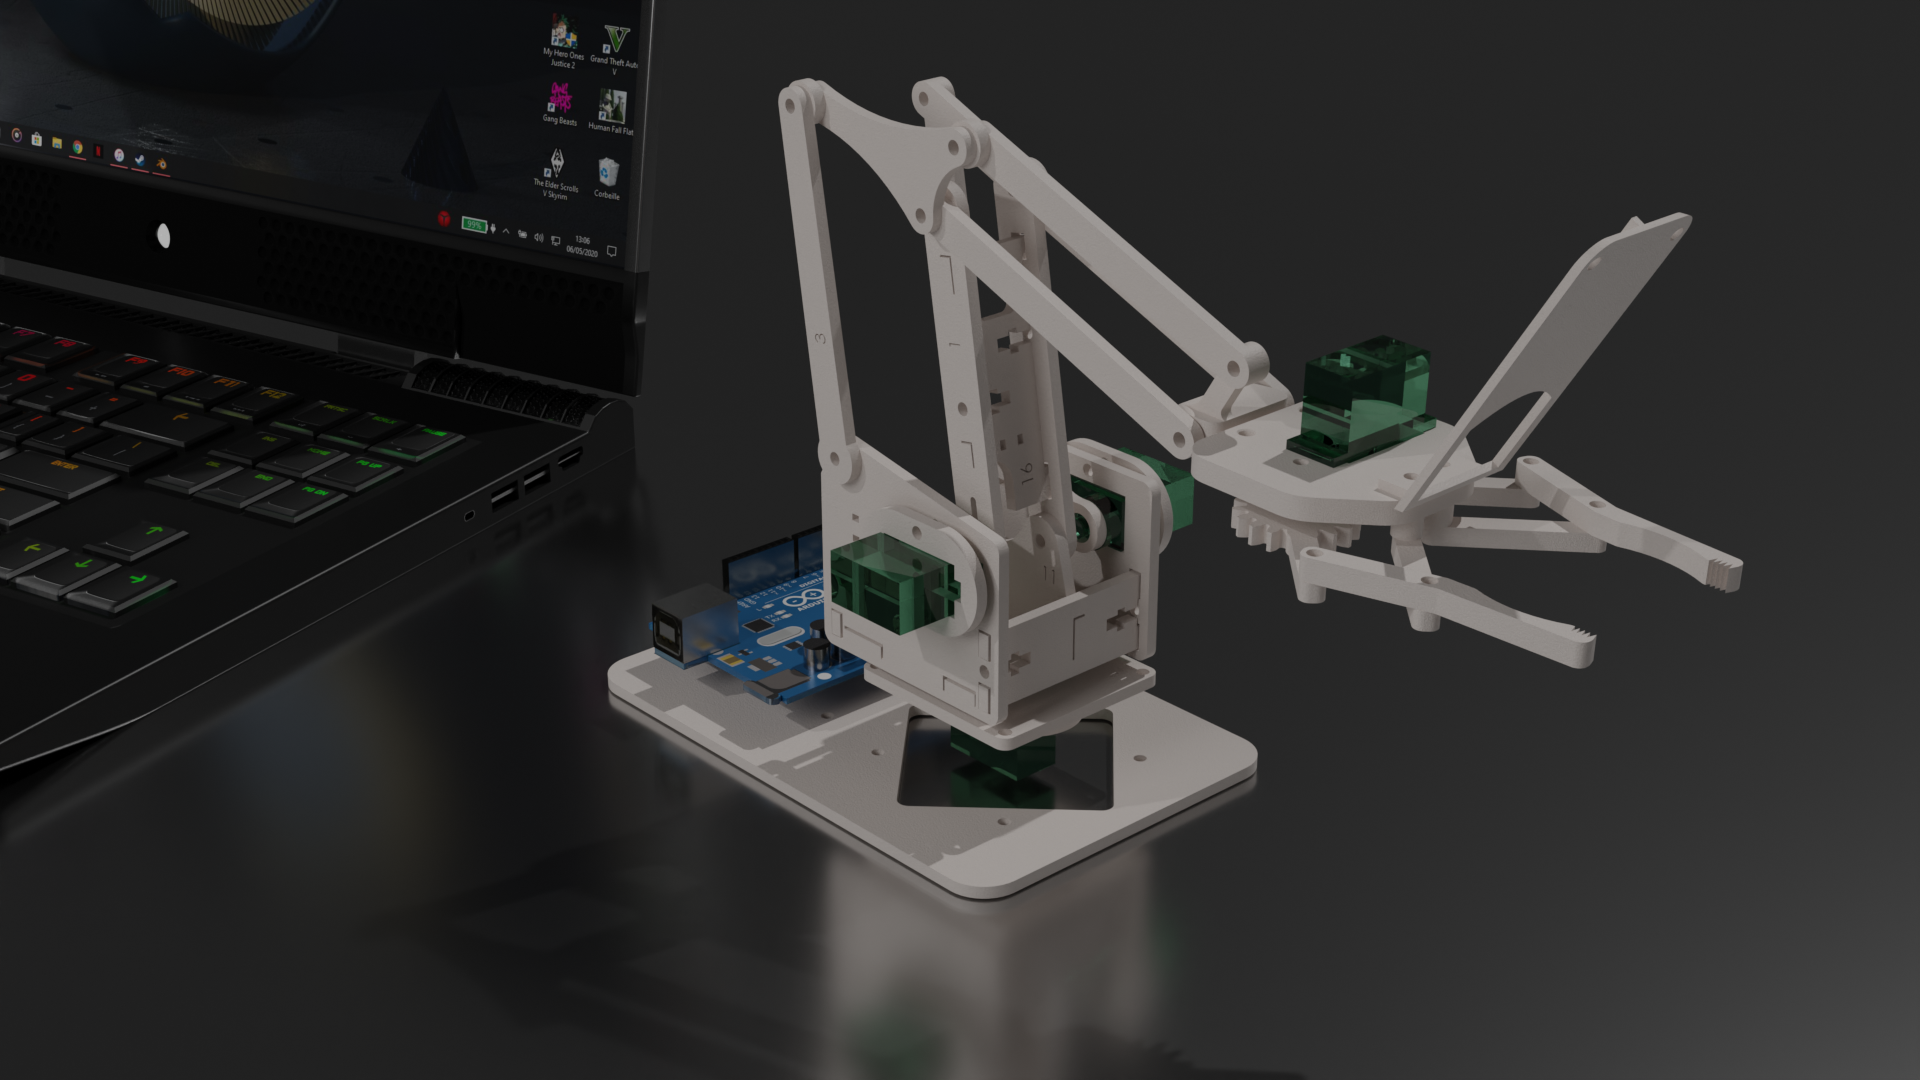
\includegraphics[width=0.95\textwidth]{mearm2.png}
    
    \vspace{1.5cm}
    
    % 底部信息（可选）
    {\fontsize{12pt}{14pt}\selectfont\color{subtitlegray}
    浙江大学学生机器人协会 · ZJUSRA\par}
    
    \vspace*{\fill}  % 下部弹性空间
\end{titlepage}

% ==================== 正文开始 ====================

\section*{前言}

    可以按照装配体文件确定零件的朝向和相对位置，本说明书只是对\textbf{安装顺序}和\textbf{注意点}进行补充说明。

\begin{figure}[h!]
    \centering
    
\includegraphics[width=0.7\textwidth]{1.png}
    \caption{装配体示意图}
\end{figure}

\section{舵机调零}
\begin{enumerate}
    \item 利用如下代码将四个舵机分别调到初始位置，旋转角度分别为 0，0，0，90，其中底座舵机的旋转角度为 90。
\end{enumerate}

\begin{lstlisting}[language=C++, caption={Arduino 舵机调零程序}, label=code:zeroing]
#include <Servo.h>

Servo servo_base;    // 底座舵机
Servo servo_arm;     // 大臂舵机
Servo servo_forearm; // 小臂舵机
Servo servo_gripper; // 夹爪舵机

// 引脚定义（请根据实际连接修改）
#define PIN_BASE    2
#define PIN_ARM     3
#define PIN_FOREARM 4
#define PIN_GRIPPER 5

void setup() {
  // 连接舵机
  servo_base.attach(PIN_BASE);
  servo_arm.attach(PIN_ARM);
  servo_forearm.attach(PIN_FOREARM);
  servo_gripper.attach(PIN_GRIPPER);

  // 设置初始角度：底座90°，其余0°
  servo_base.write(90);
  servo_arm.write(0);
  servo_forearm.write(0);
  servo_gripper.write(0);
}

void loop() {
  // 无需重复执行
}
\end{lstlisting}

\begin{enumerate}
    \setcounter{enumi}{1}
    \item 利用图 \ref{fig:screw} 中自攻螺钉安装舵机臂与传动臂。
\end{enumerate}

% 图2 + 图3 并排
\begin{figure}[h!]
    \centering
    \begin{minipage}[b]{0.45\textwidth}
        \centering
        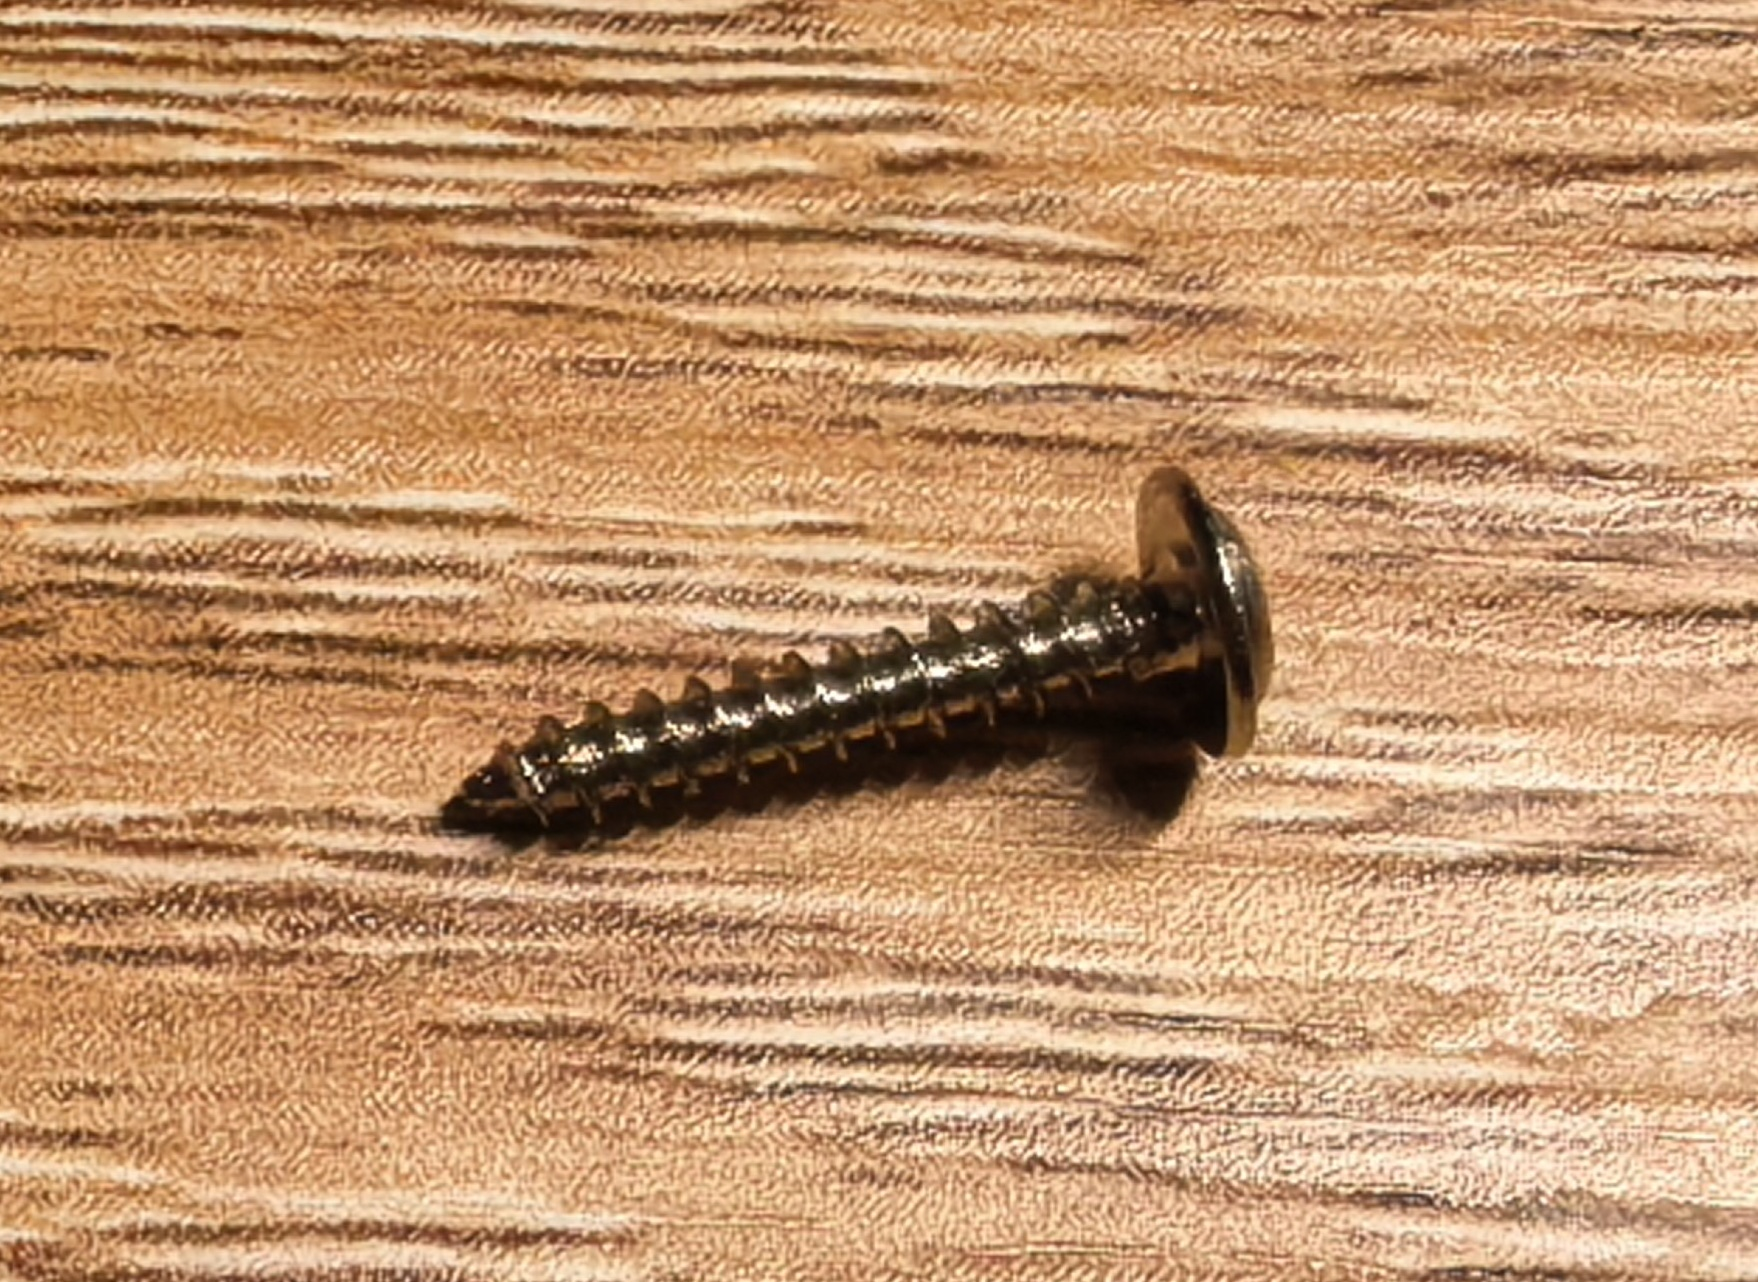
\includegraphics[width=\linewidth]{IMG_20260301_114419.jpg}
        \caption{自攻螺钉安装示意}
        \label{fig:screw}
    \end{minipage}
    \hfill
    \begin{minipage}[b]{0.45\textwidth}
        \centering
        \includegraphics[width=\linewidth]{IMG_20260301_114800.jpg}
        \caption{四个舵机臂与传动臂}
        \label{fig:fourarms}
    \end{minipage}
\end{figure}

四个舵机分别对应四个舵机臂与传动臂，故需安装四个，如图 \ref{fig:fourarms} 和图 \ref{fig:mountway}：

% 图4 + 图5 并排
\begin{figure}[h!]
    \centering
    \begin{minipage}[b]{0.45\textwidth}
        \centering
        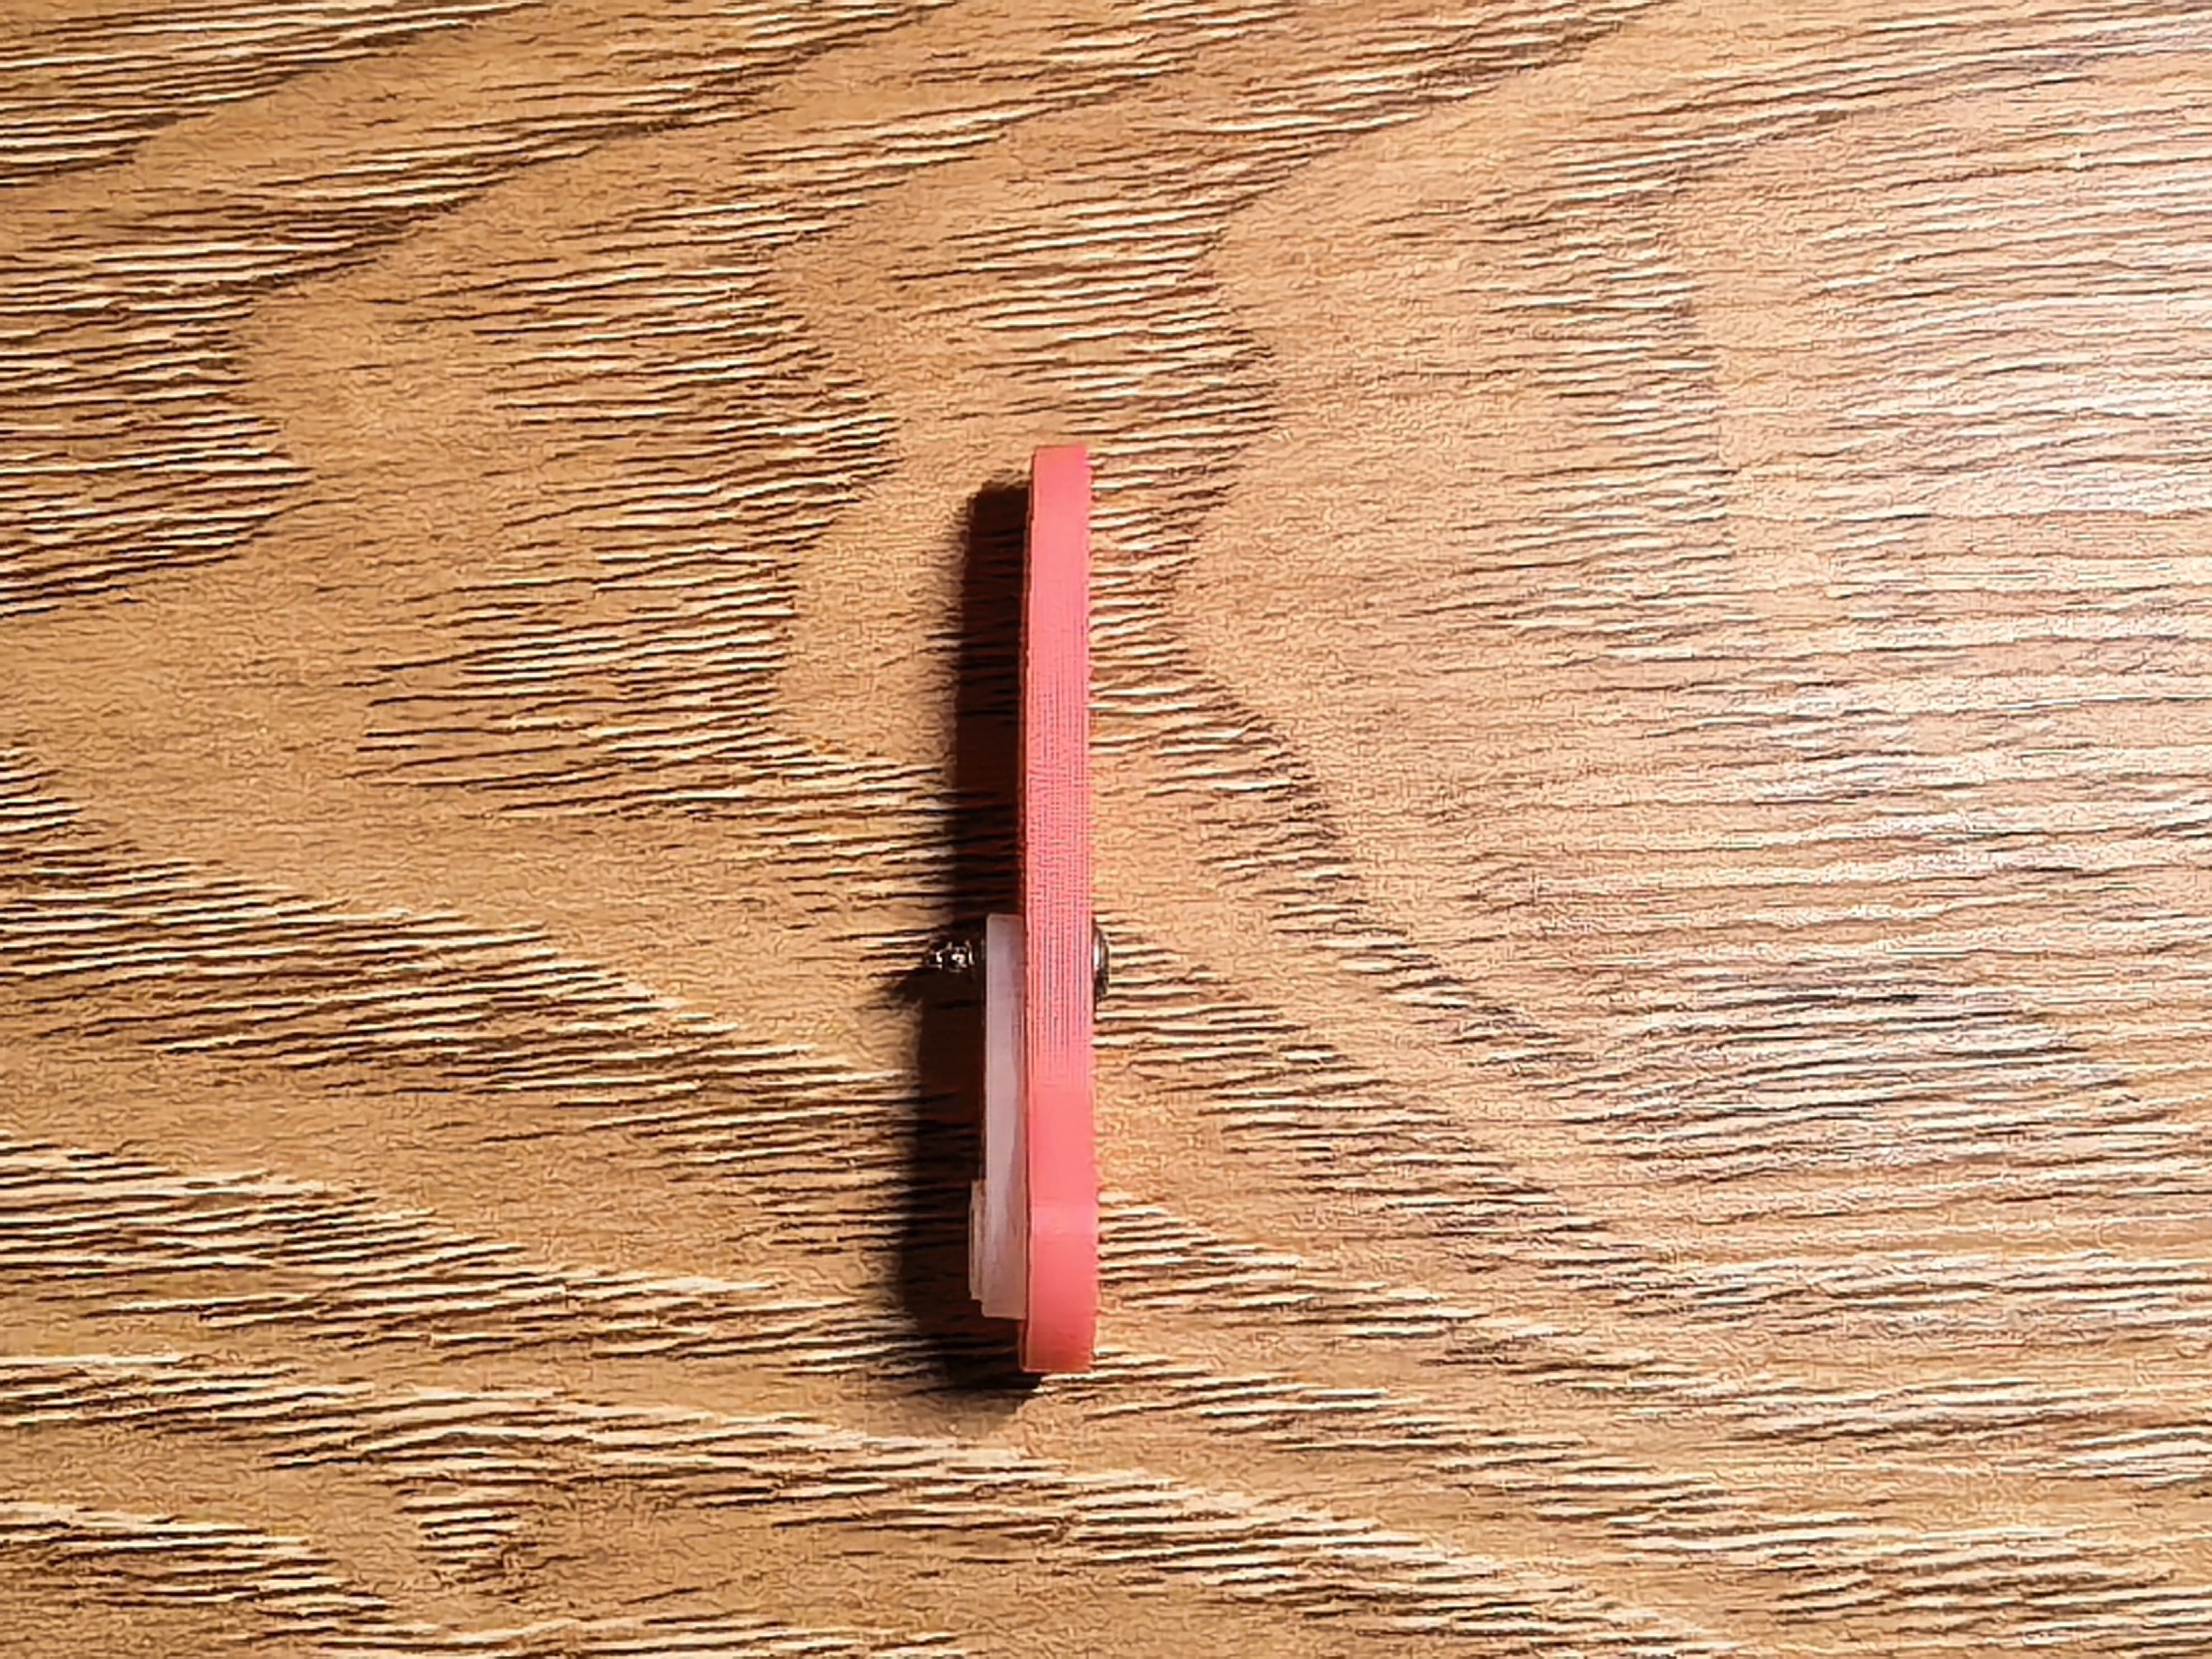
\includegraphics[width=\linewidth]{IMG_20260301_114841.jpg}
        \caption{安装方式示意}
        \label{fig:mountway}
    \end{minipage}
    \hfill
    \begin{minipage}[b]{0.45\textwidth}
        \centering
        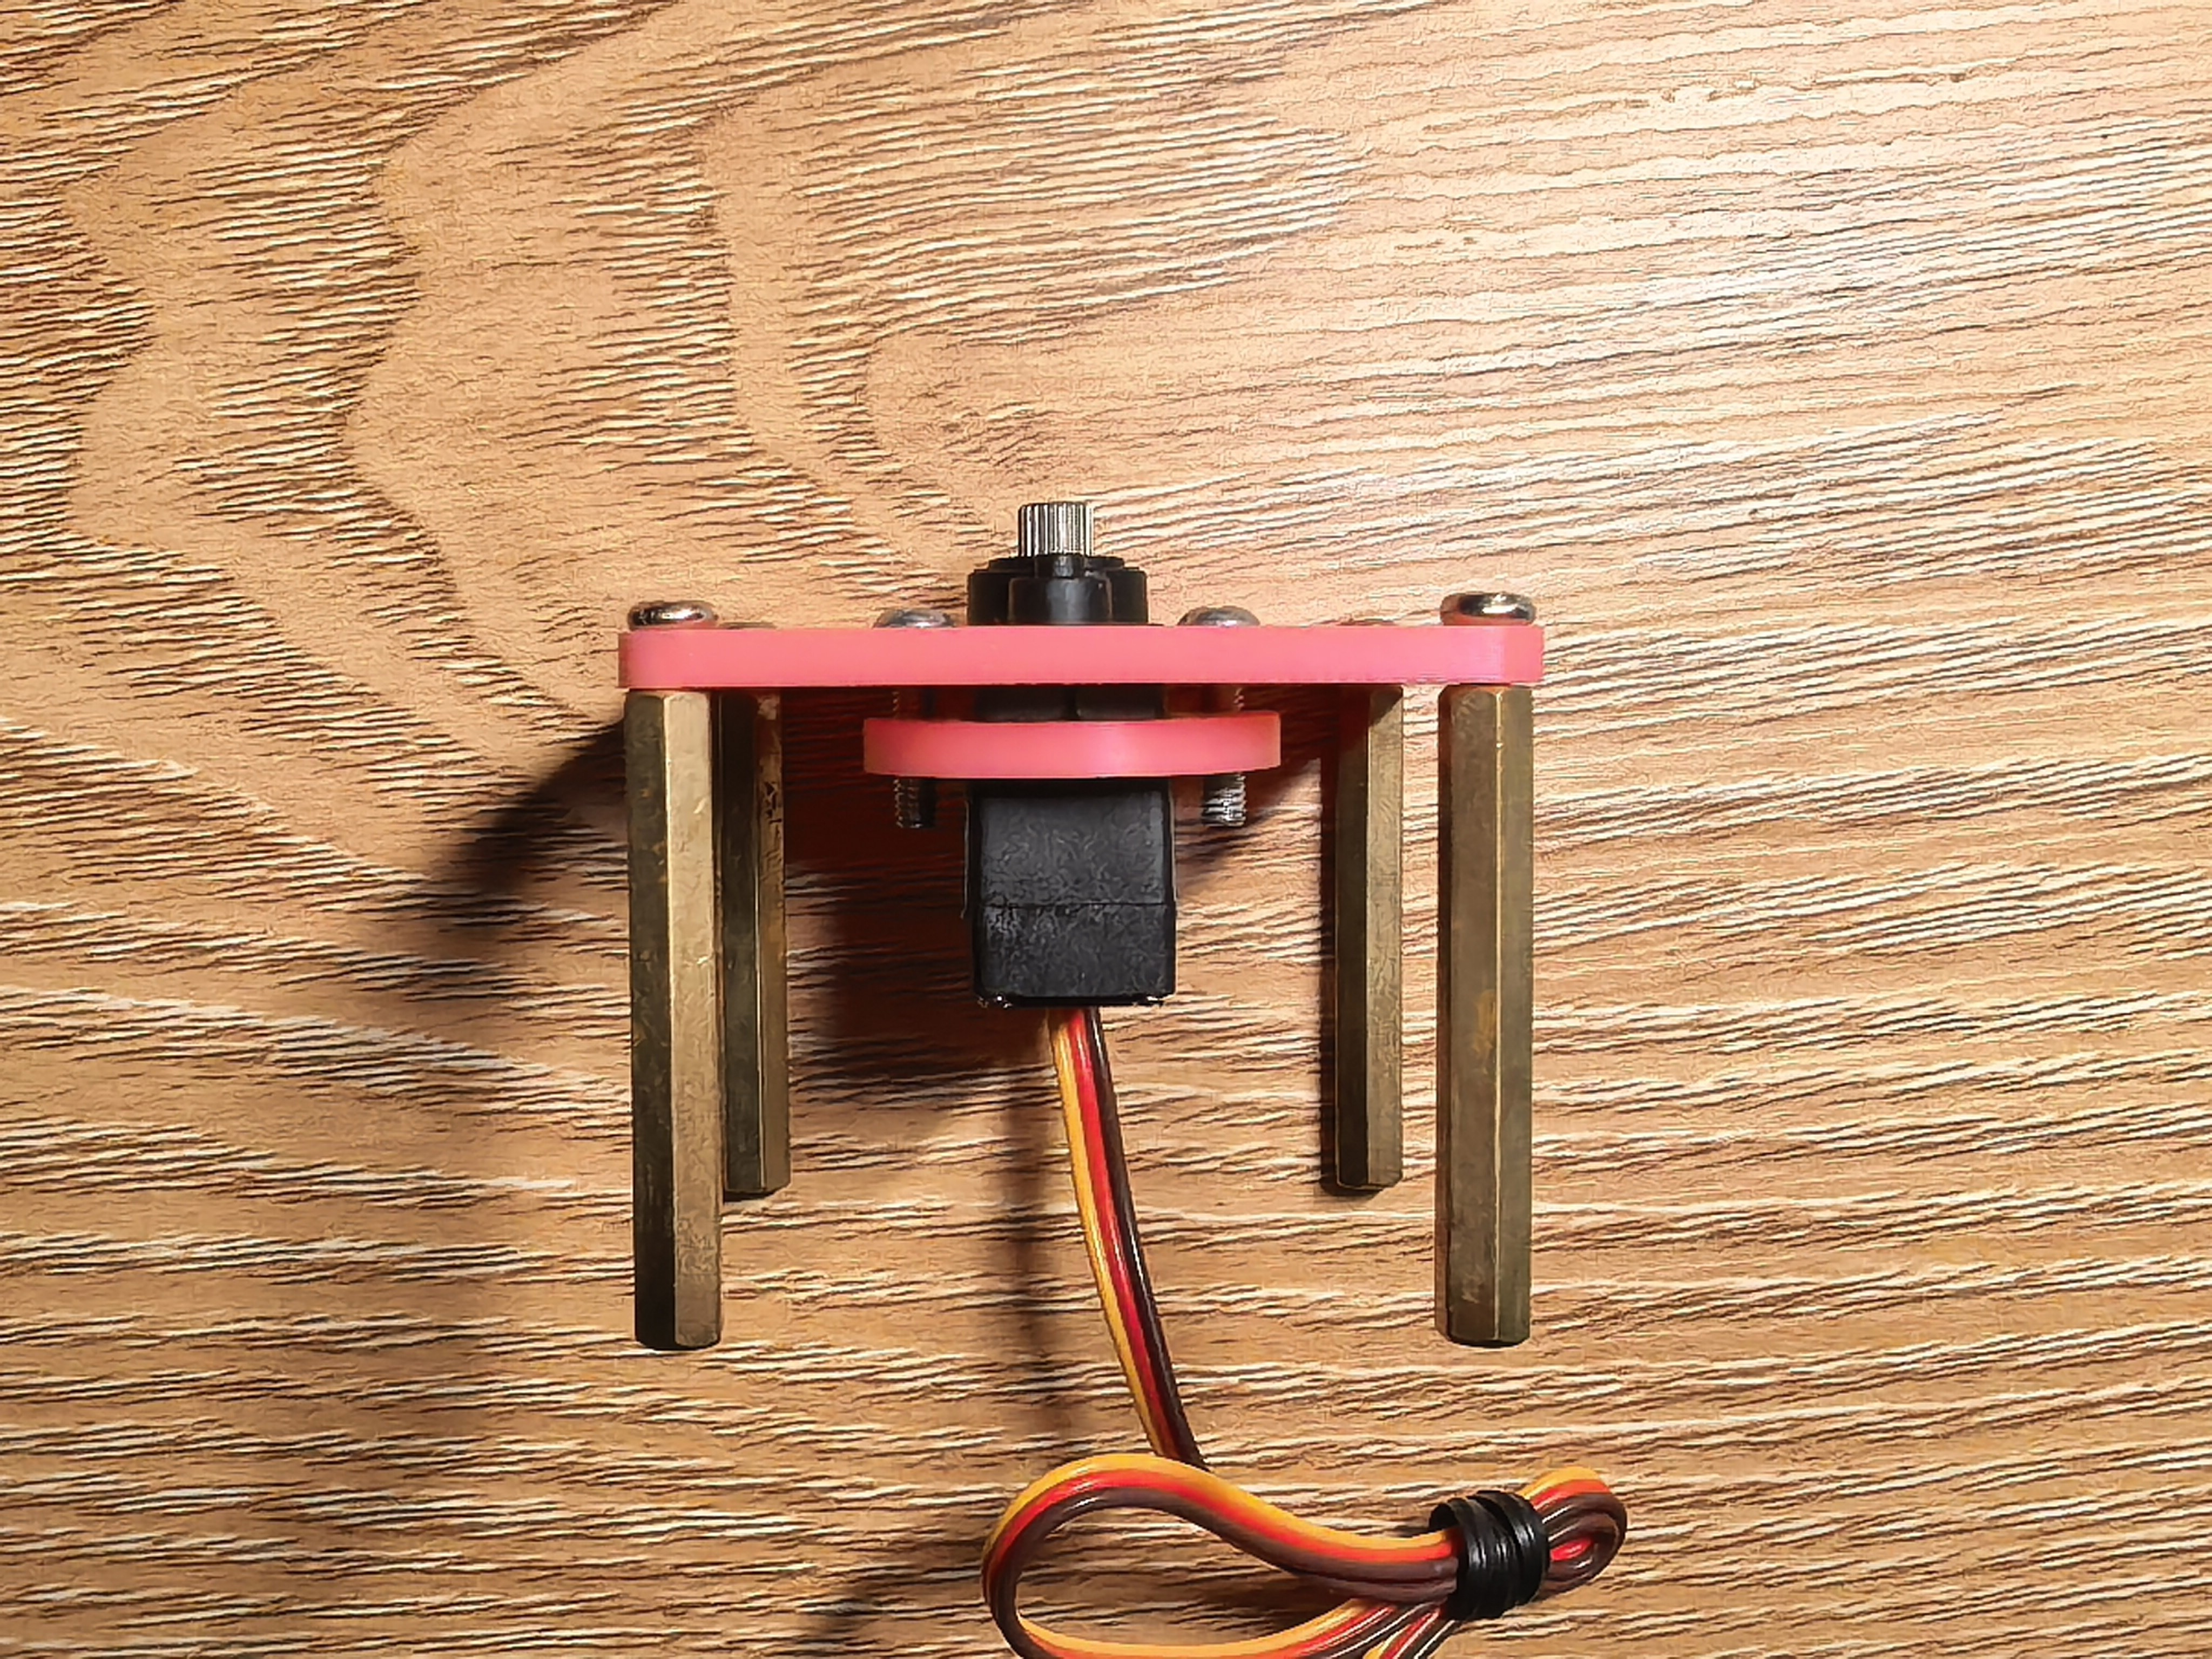
\includegraphics[width=\linewidth]{IMG_20260301_114133.jpg}
        \caption{底座舵机固定}
    \end{minipage}
\end{figure}

\section{安装底座舵机和底座}
\textbf{注意：安装前请确认底座舵机目前的转动角度为 90°！}

\begin{enumerate}
    \item 利用舵机安装板固定底座舵机，并安装四个铜柱。
    \begin{itemize}
        \item 具体零件可以看装配体文件。
    \end{itemize}
\end{enumerate}

\begin{enumerate}
    \setcounter{enumi}{1}
    \item 将舵机臂与舵机连接，注意按照图 \ref{fig:basearm} 中朝向安装。
\end{enumerate}

% 图6 + 图7 并排
\begin{figure}[h!]
    \centering
    \begin{minipage}[b]{0.45\textwidth}
        \centering
        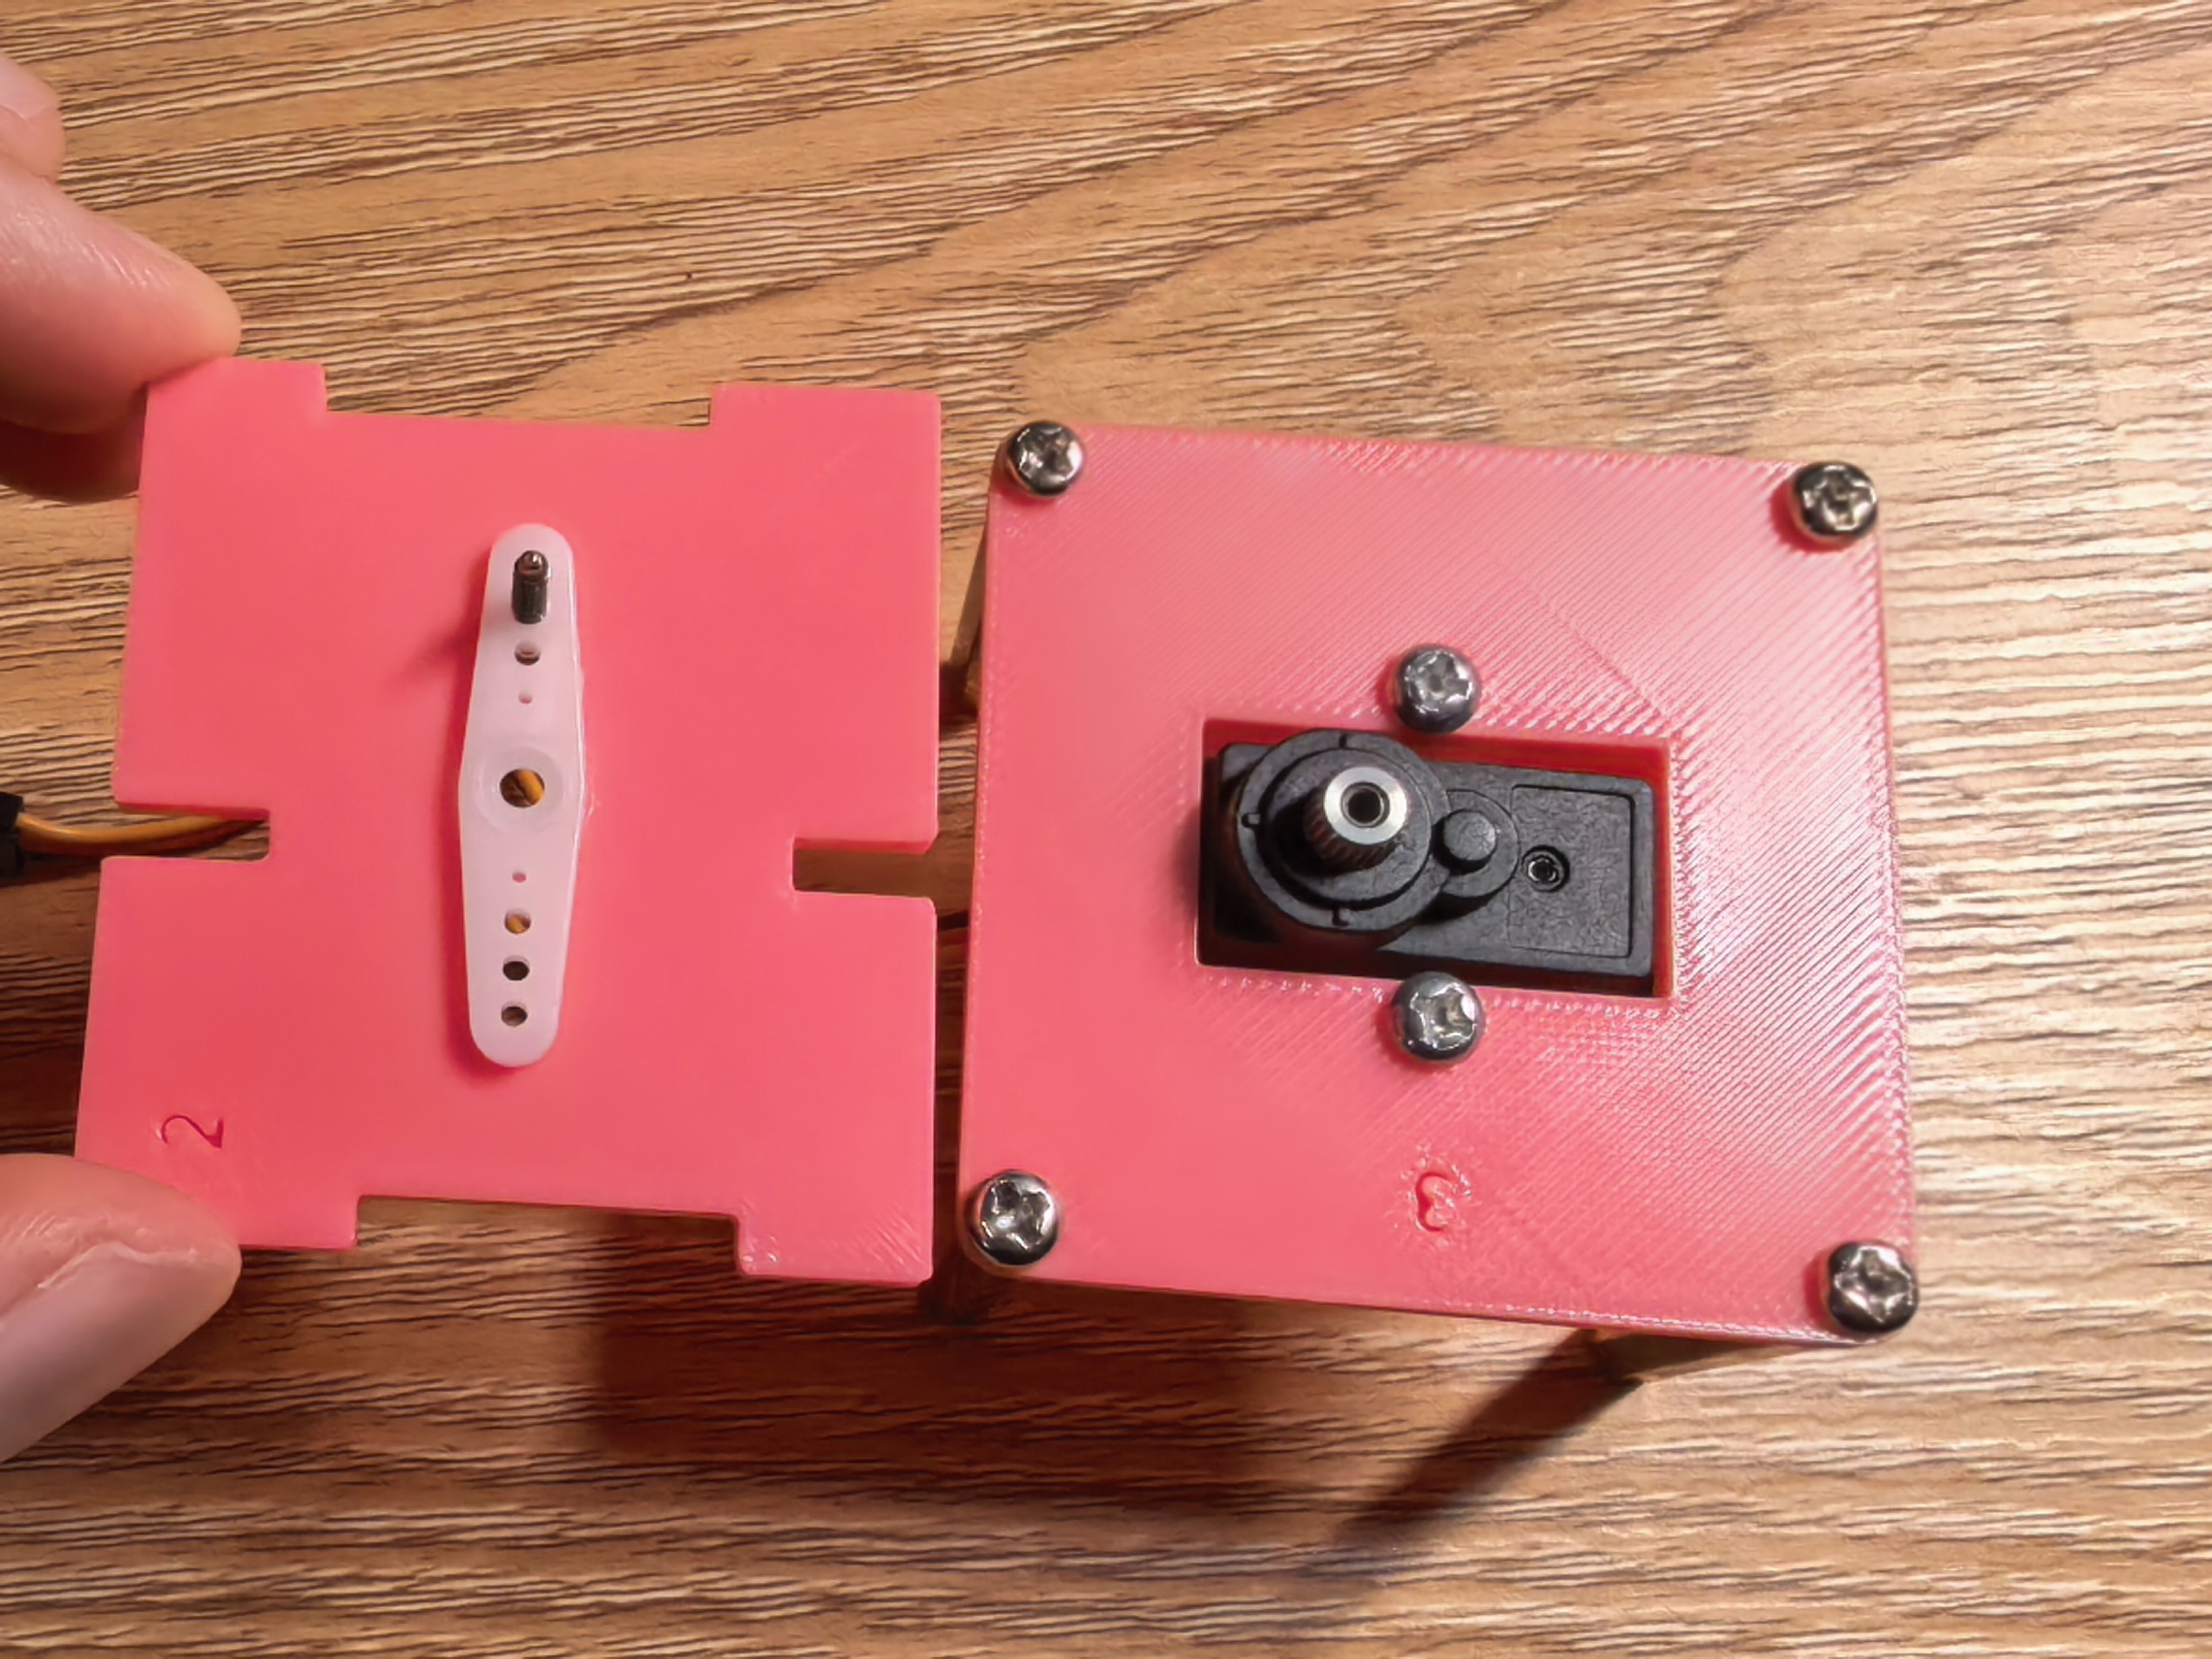
\includegraphics[width=\linewidth]{IMG_20260301_120743.jpg}
        \caption{舵机臂朝向}
        \label{fig:basearm}
    \end{minipage}
    \hfill
    \begin{minipage}[b]{0.45\textwidth}
        \centering
        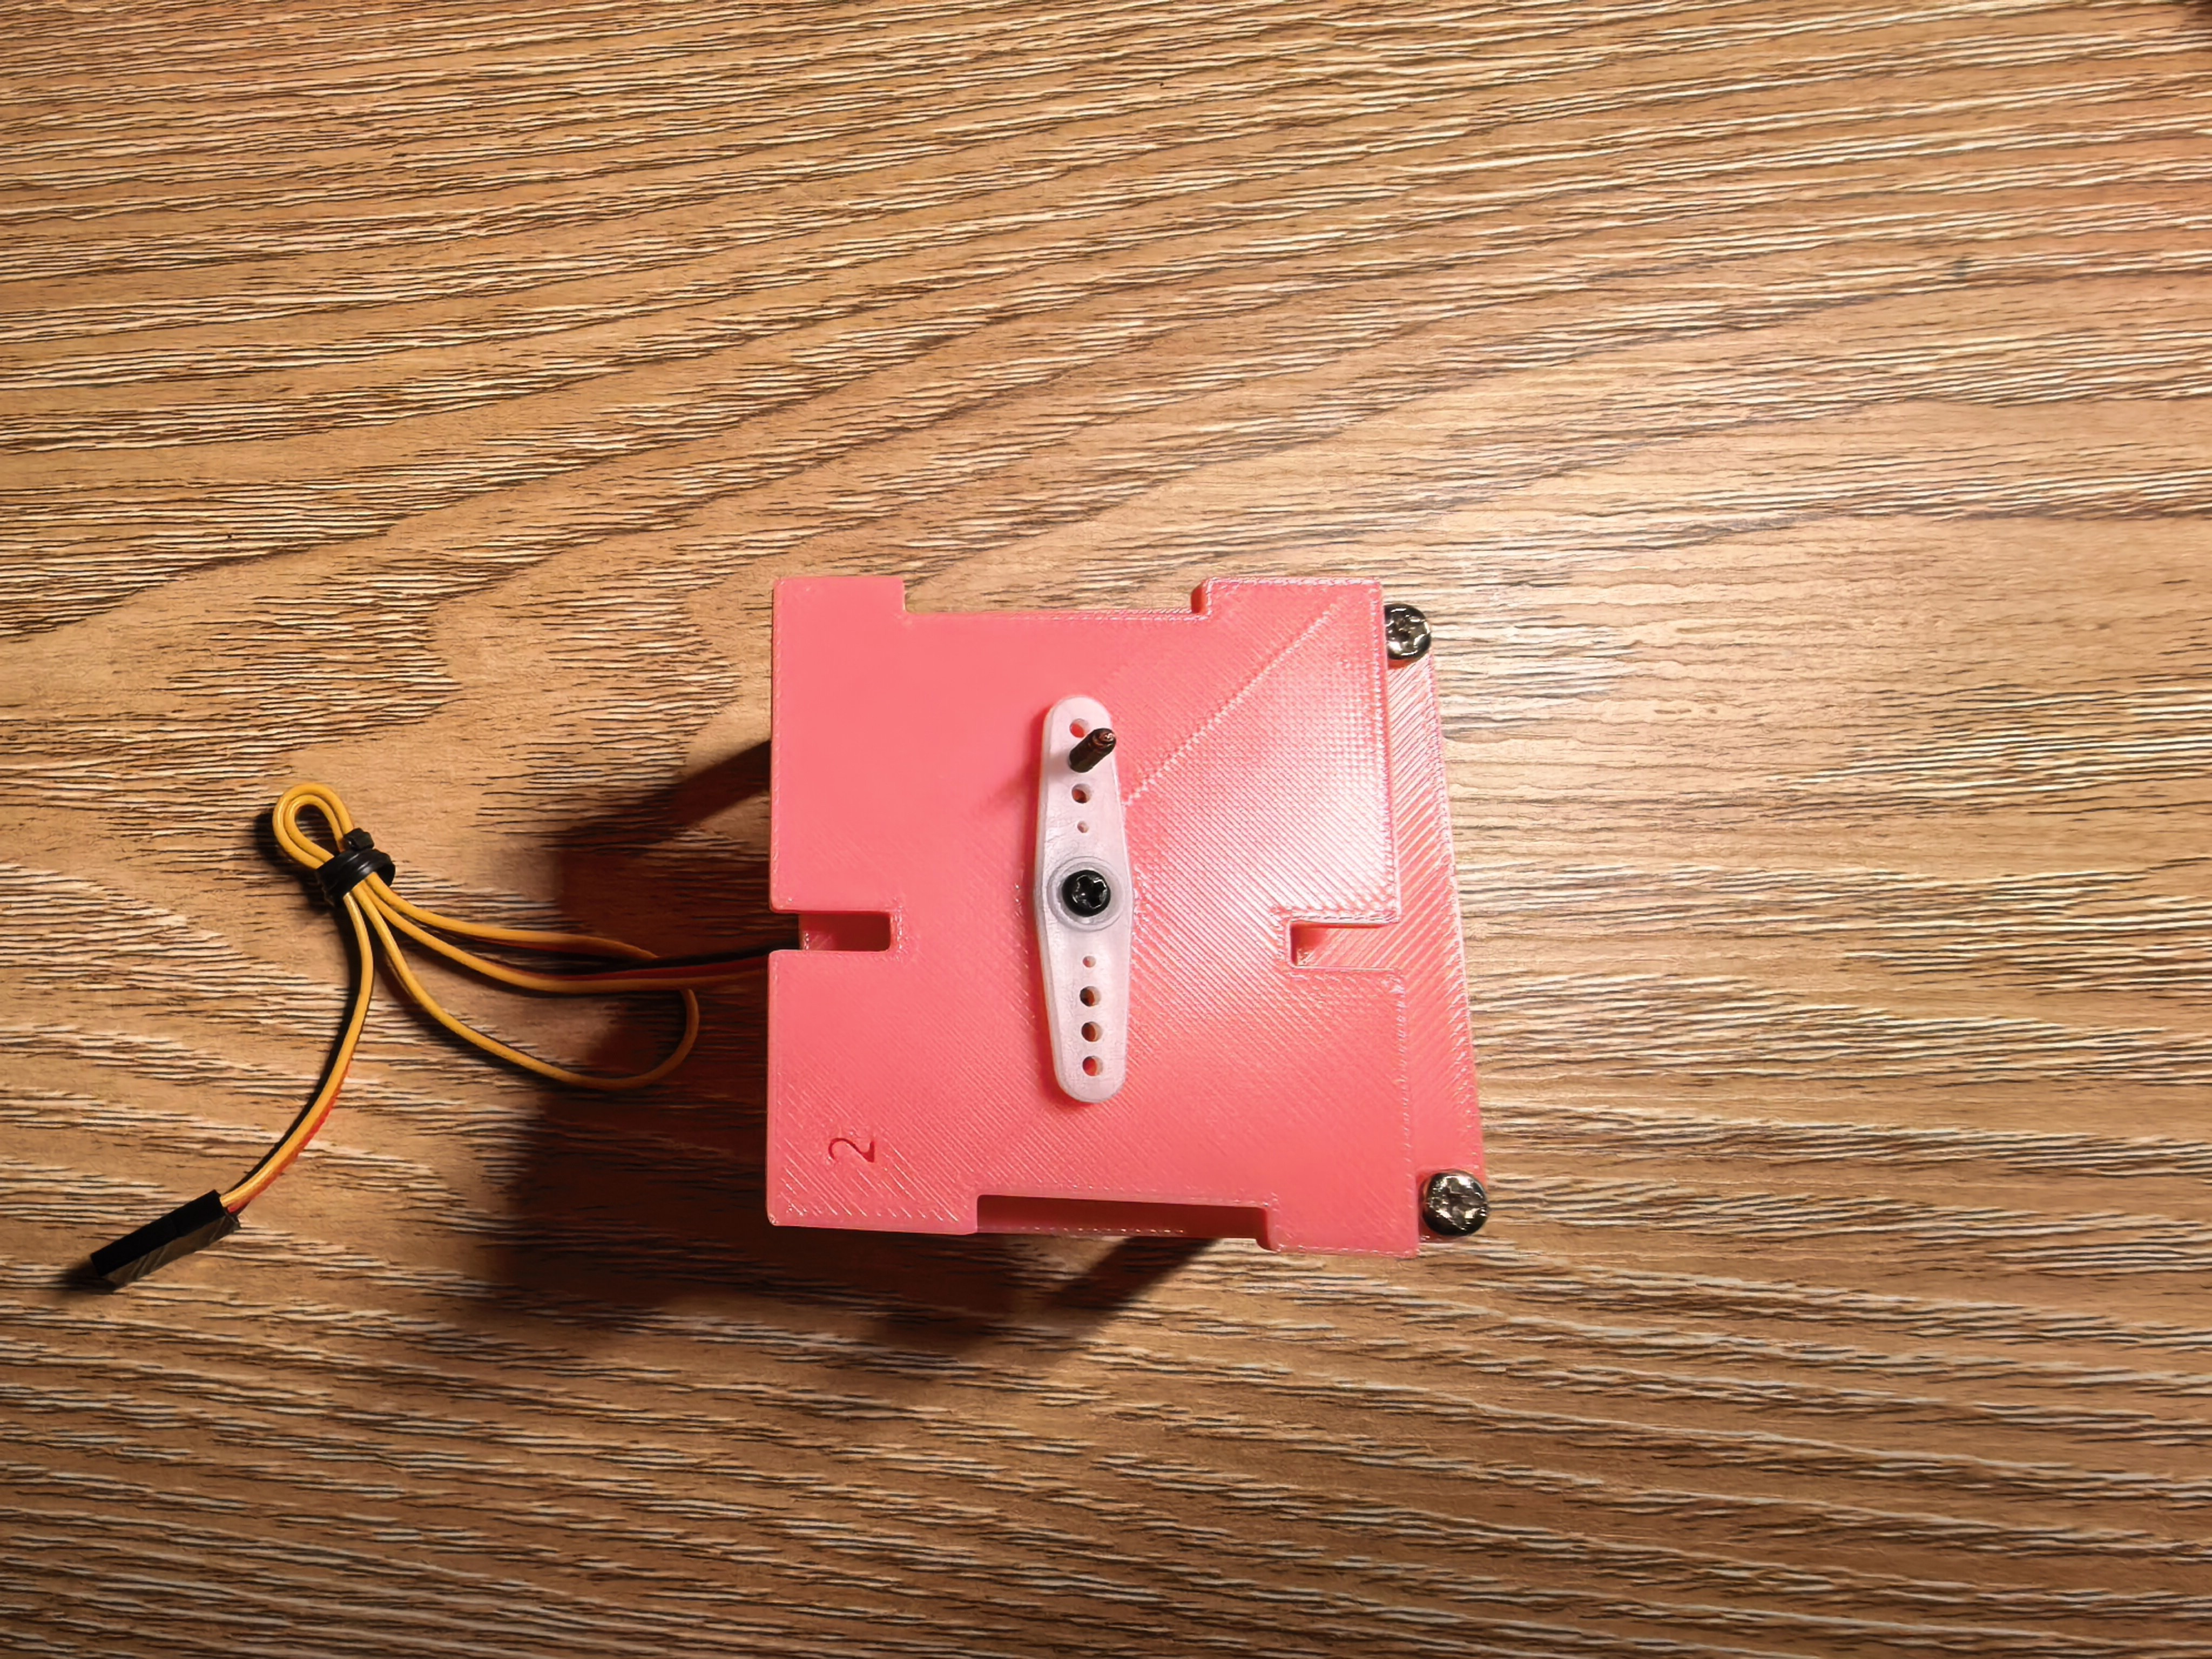
\includegraphics[width=\linewidth]{IMG_20260301_121030.jpg}
        \caption{拧紧小螺丝}
    \end{minipage}
\end{figure}

\section{安装大臂}
\textbf{注意：安装前确认大臂舵机的旋转角为 0°！}

\begin{enumerate}
    \item 利用同样的方式（也就是用舵机安装板）将大臂舵机安装在侧壁上，再按如图 \ref{fig:bigarm} 角度安装舵机臂，并拧上小螺丝。
\end{enumerate}

% 图8 + 图9 并排
\begin{figure}[h!]
    \centering
    \begin{minipage}[b]{0.45\textwidth}
        \centering
        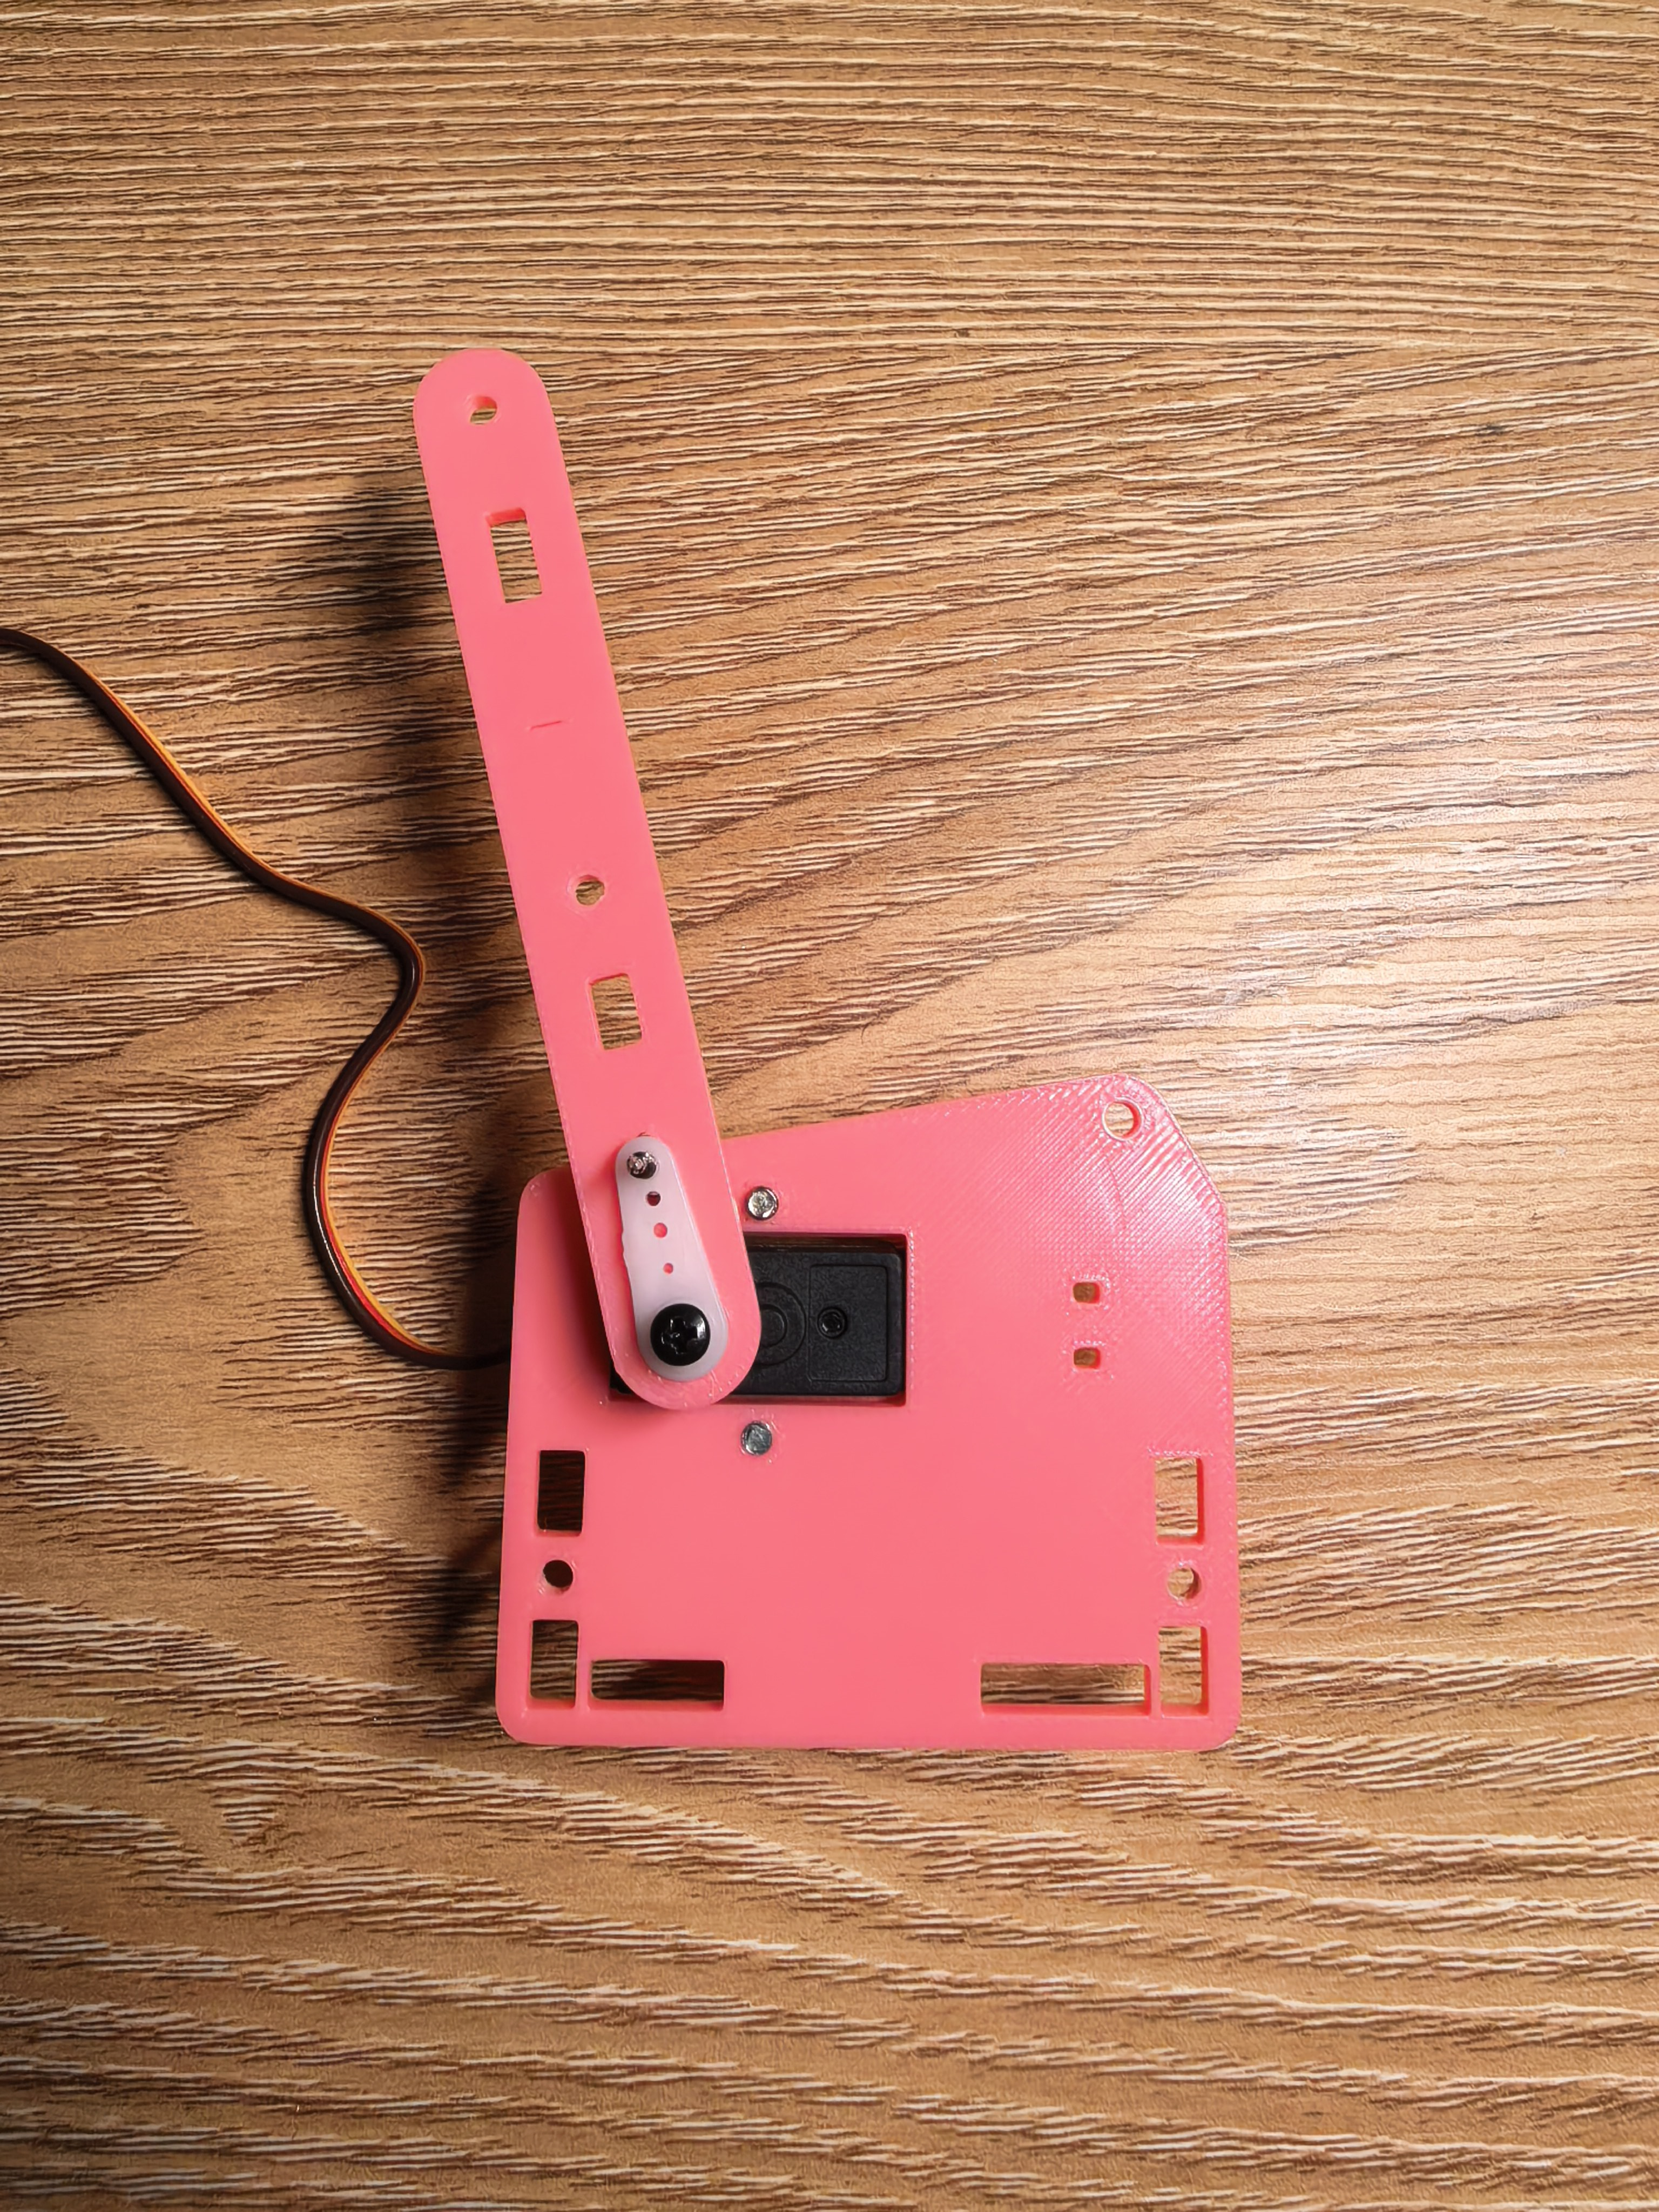
\includegraphics[width=\linewidth]{IMG_20260301_121703.jpg}
        \caption{大臂舵机安装}
        \label{fig:bigarm}
    \end{minipage}
    \hfill
    \begin{minipage}[b]{0.45\textwidth}
        \centering
        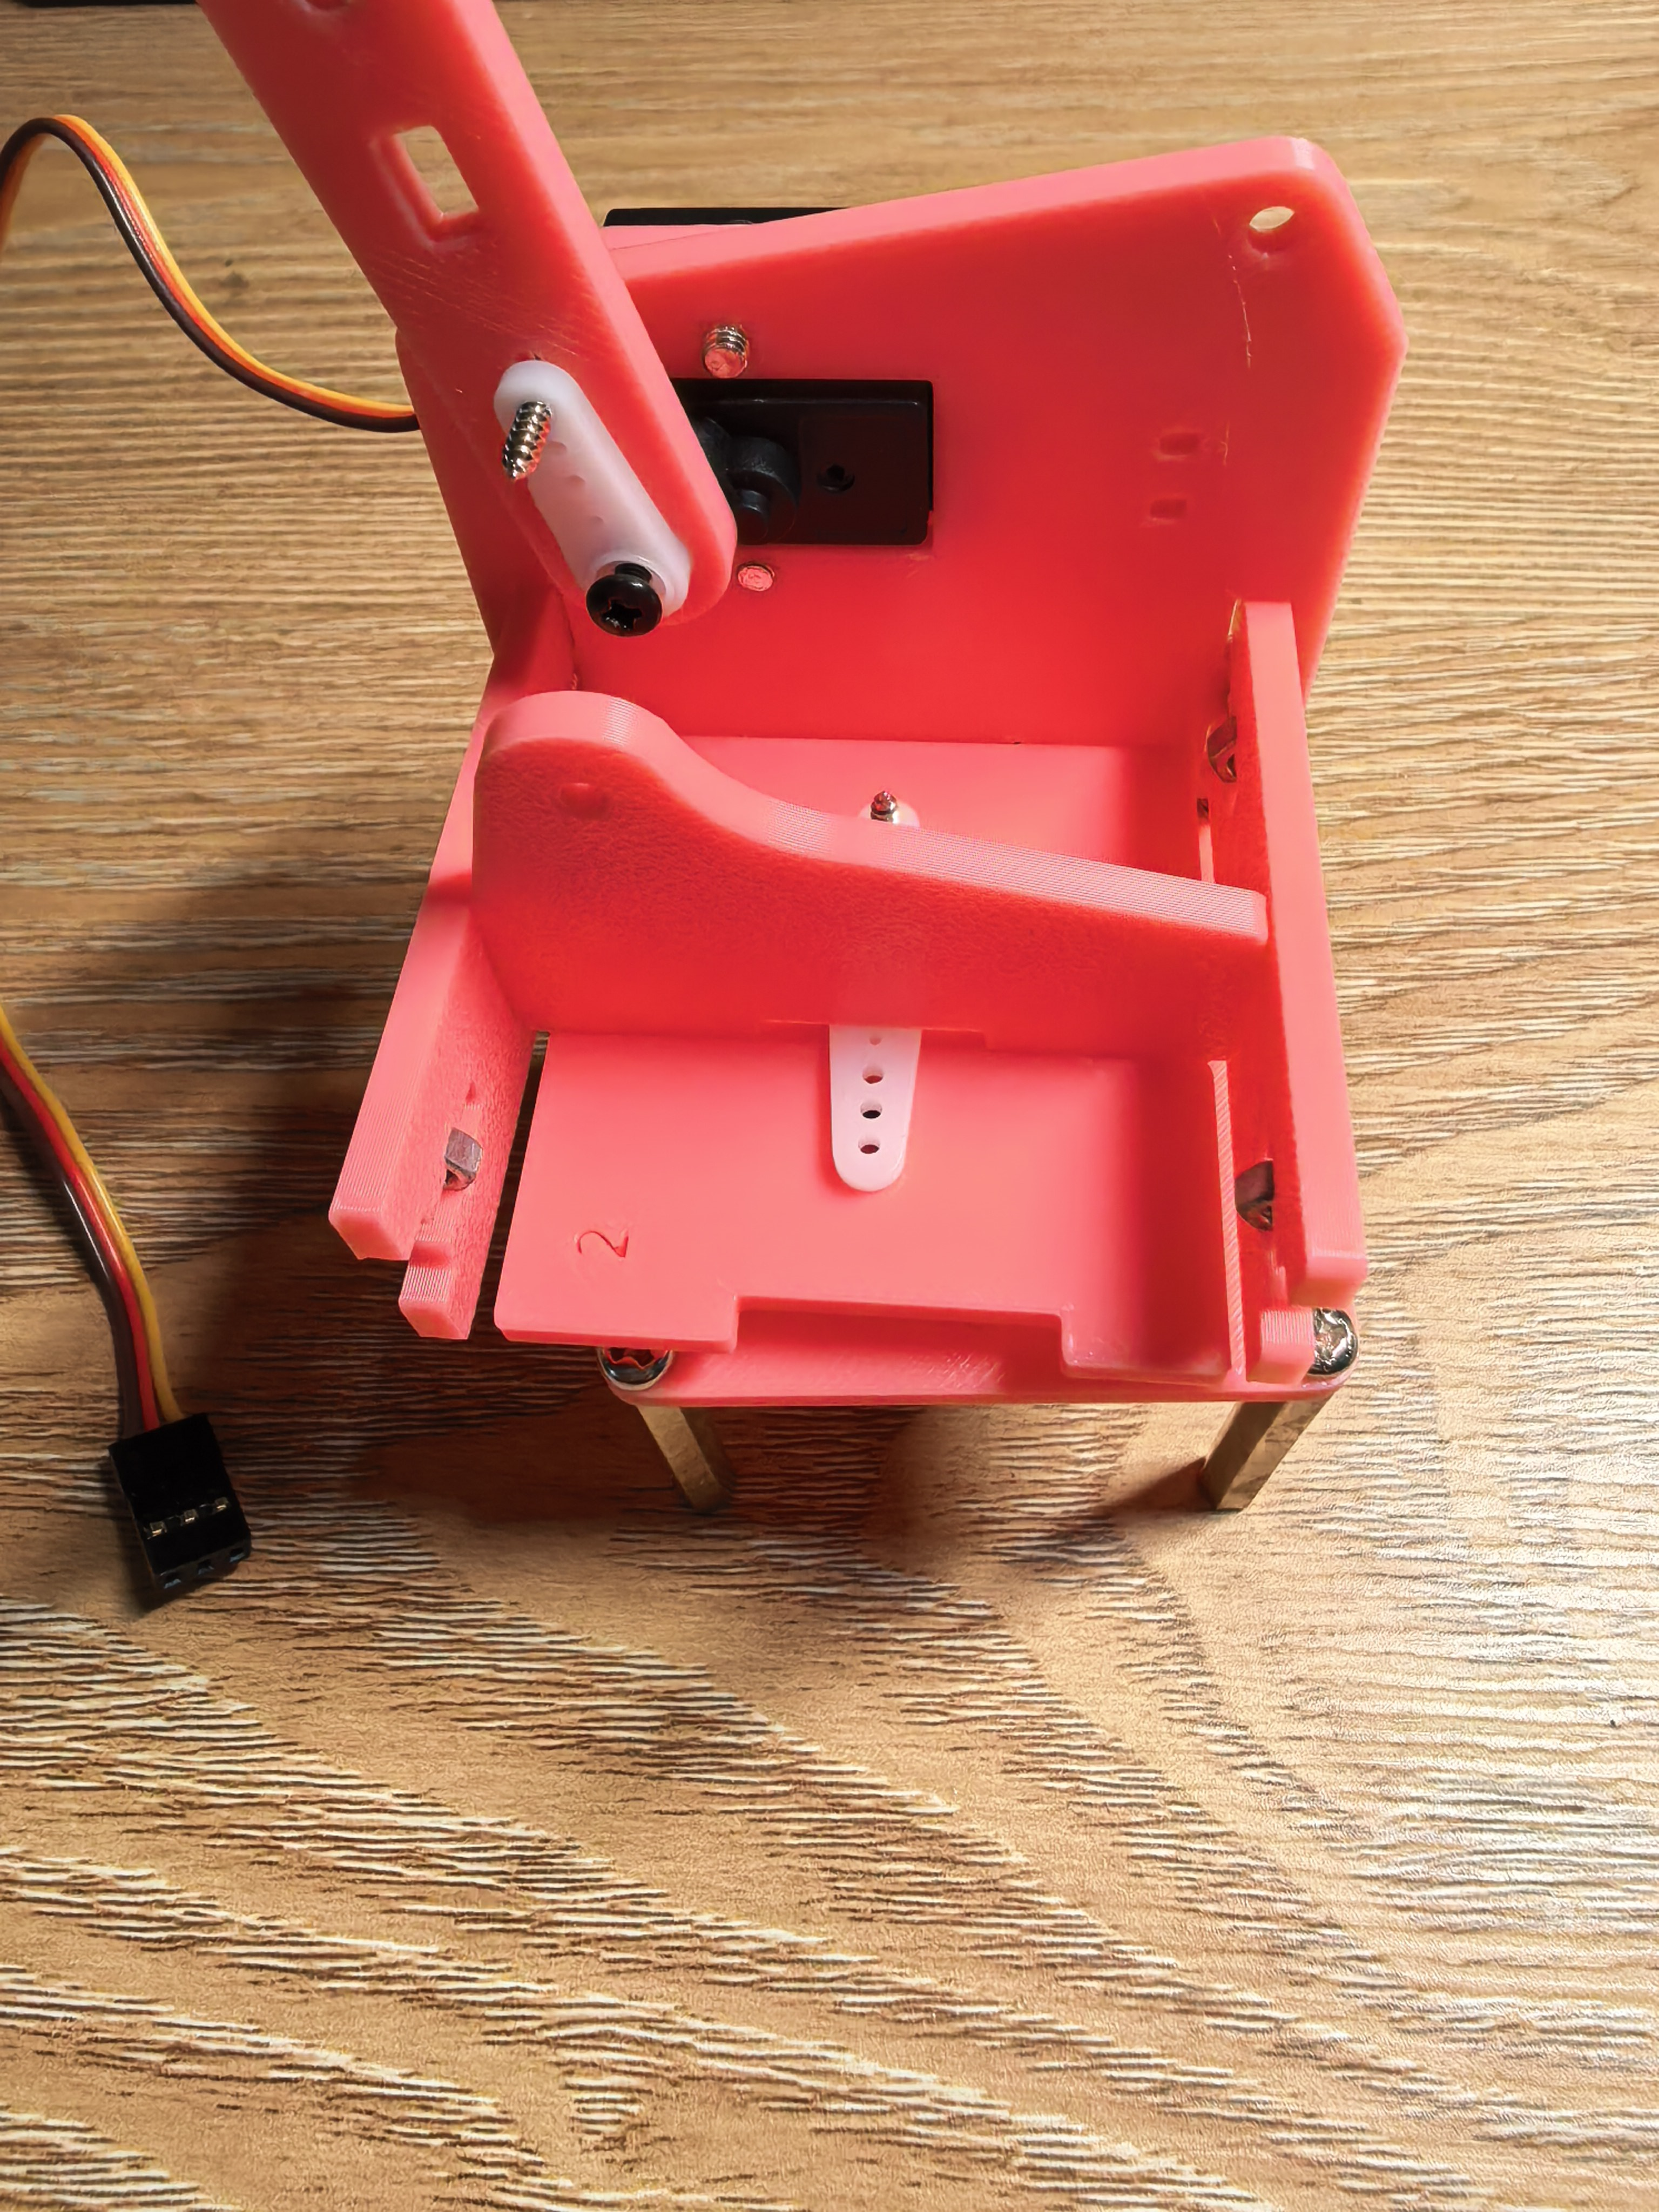
\includegraphics[width=\linewidth]{IMG_20260301_121926.jpg}
        \caption{转台侧壁和大臂安装座}
        \label{fig:sides}
    \end{minipage}
\end{figure}

\begin{enumerate}
    \setcounter{enumi}{1}
    \item 安装两个转台侧壁和大臂安装座（图 \ref{fig:sides} 中三个零件）。
\end{enumerate}

注意需要用螺丝螺母固定，如图 \ref{fig:screwnut}：

% 图10 + 图11 并排
\begin{figure}[h!]
    \centering
    \begin{minipage}[b]{0.45\textwidth}
        \centering
        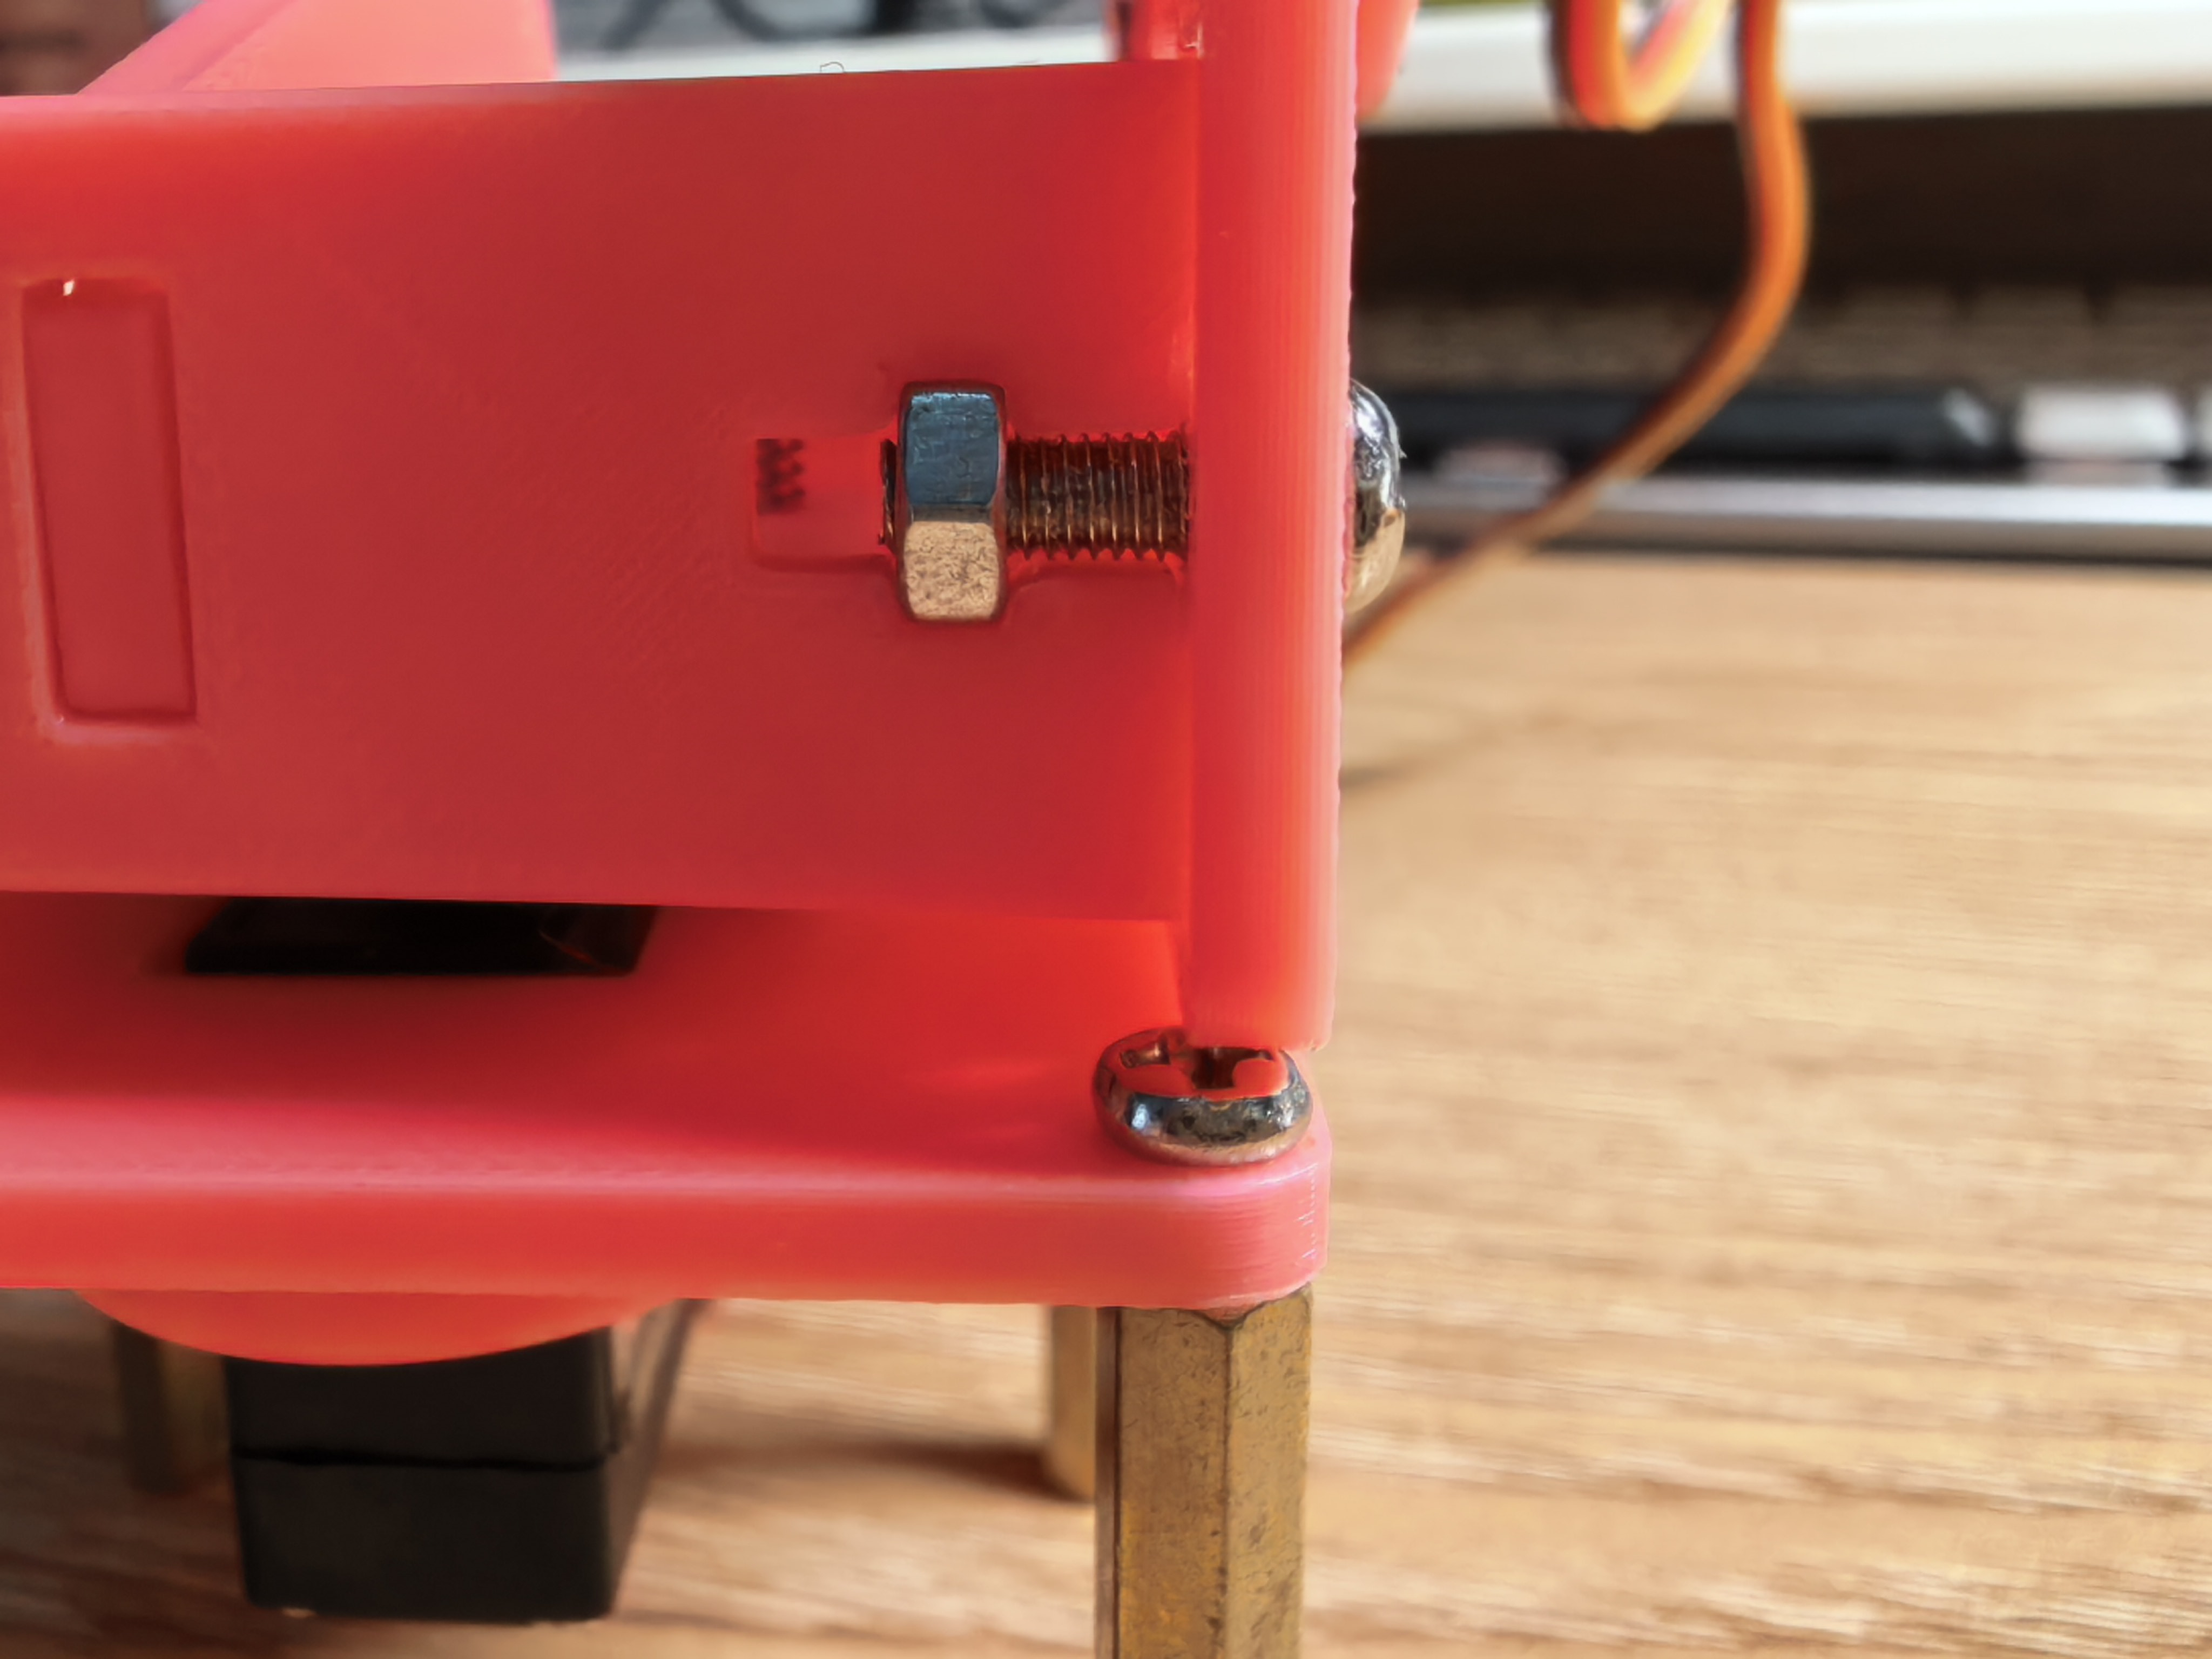
\includegraphics[width=\linewidth]{IMG_20260301_121235.jpg}
        \caption{螺丝螺母固定}
        \label{fig:screwnut}
    \end{minipage}
    \hfill
    \begin{minipage}[b]{0.45\textwidth}
        \centering
        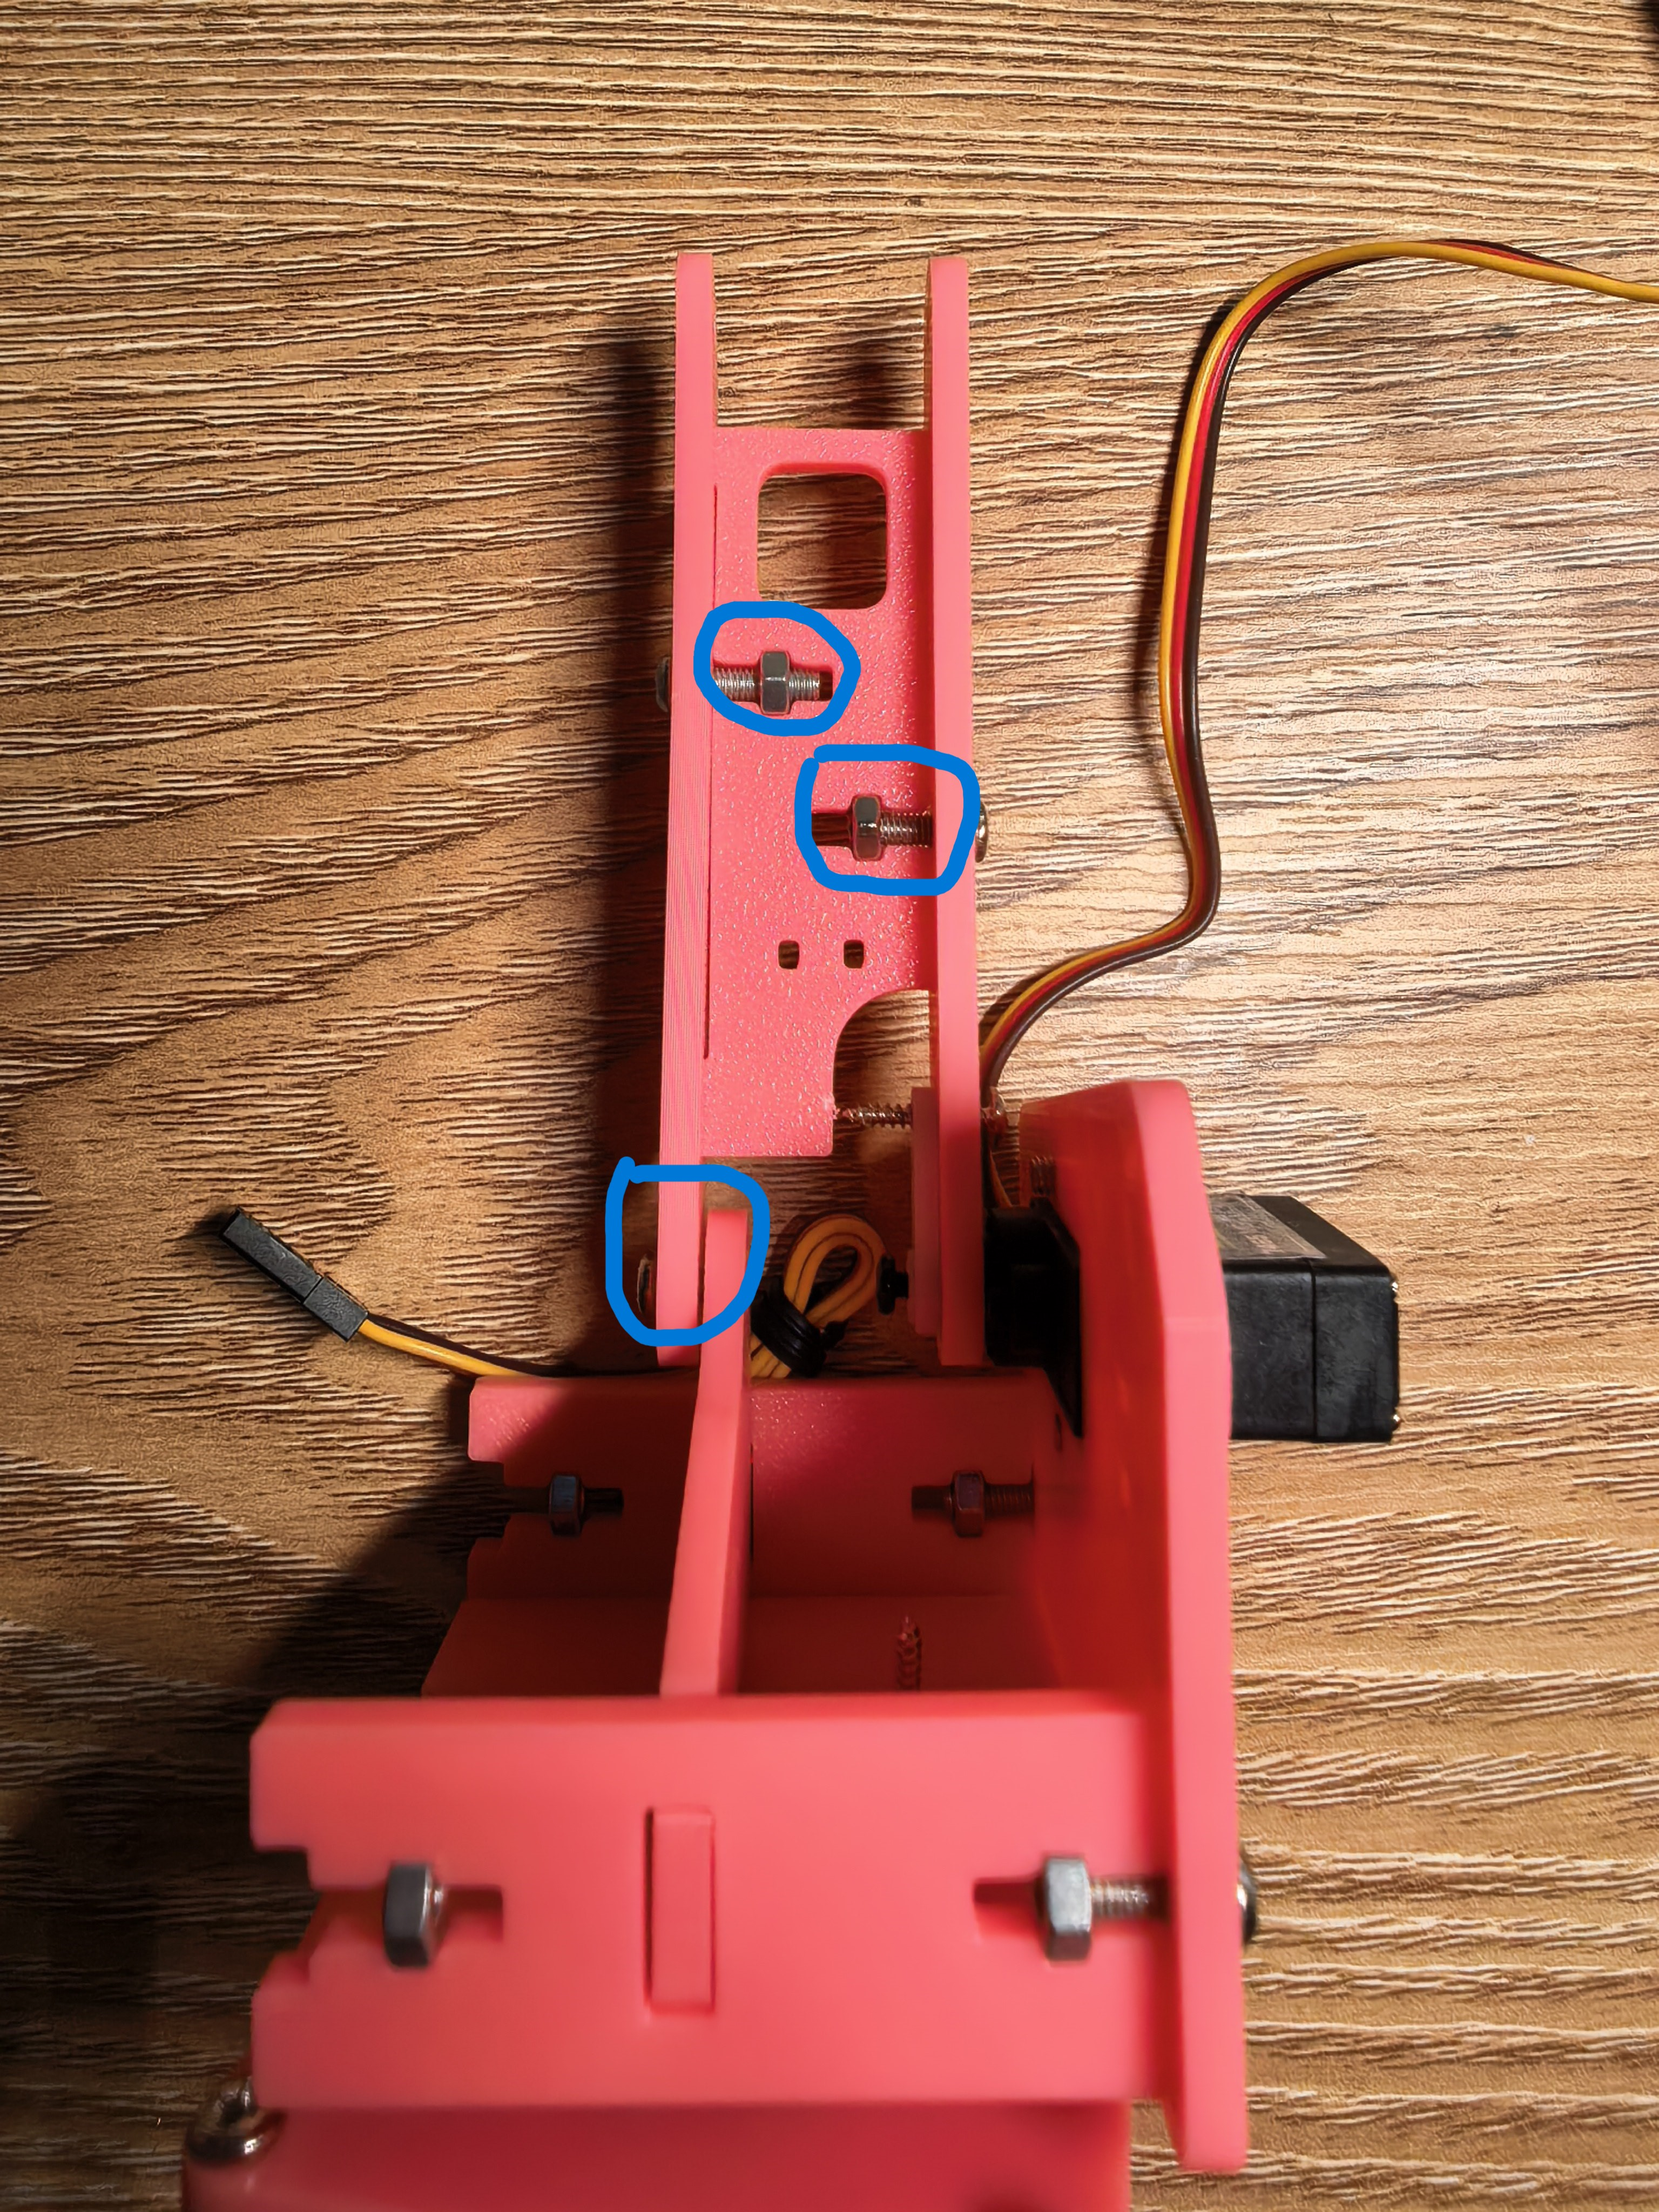
\includegraphics[width=\linewidth]{IMG_20260301_122302.jpg}
        \caption{大臂整体安装}
        \label{fig:fullarm}
    \end{minipage}
\end{figure}

\begin{enumerate}
    \setcounter{enumi}{2}
    \item 安装整个大臂，注意共三个需要螺钉连接的地方（图 \ref{fig:fullarm}）。
\end{enumerate}

\newpage
\section{安装小臂}
\textbf{注意：安装前确认小臂舵机的旋转角为 0°！}

\begin{enumerate}
    \item 同样，利用舵机安装板安装小臂舵机、侧壁，并在内侧安装舵机臂，注意参照图 \ref{fig:smallarm} 中角度！
\end{enumerate}

% 图12 + 图13 并排
\begin{figure}[h!]
    \centering
    \begin{minipage}[b]{0.45\textwidth}
        \centering
        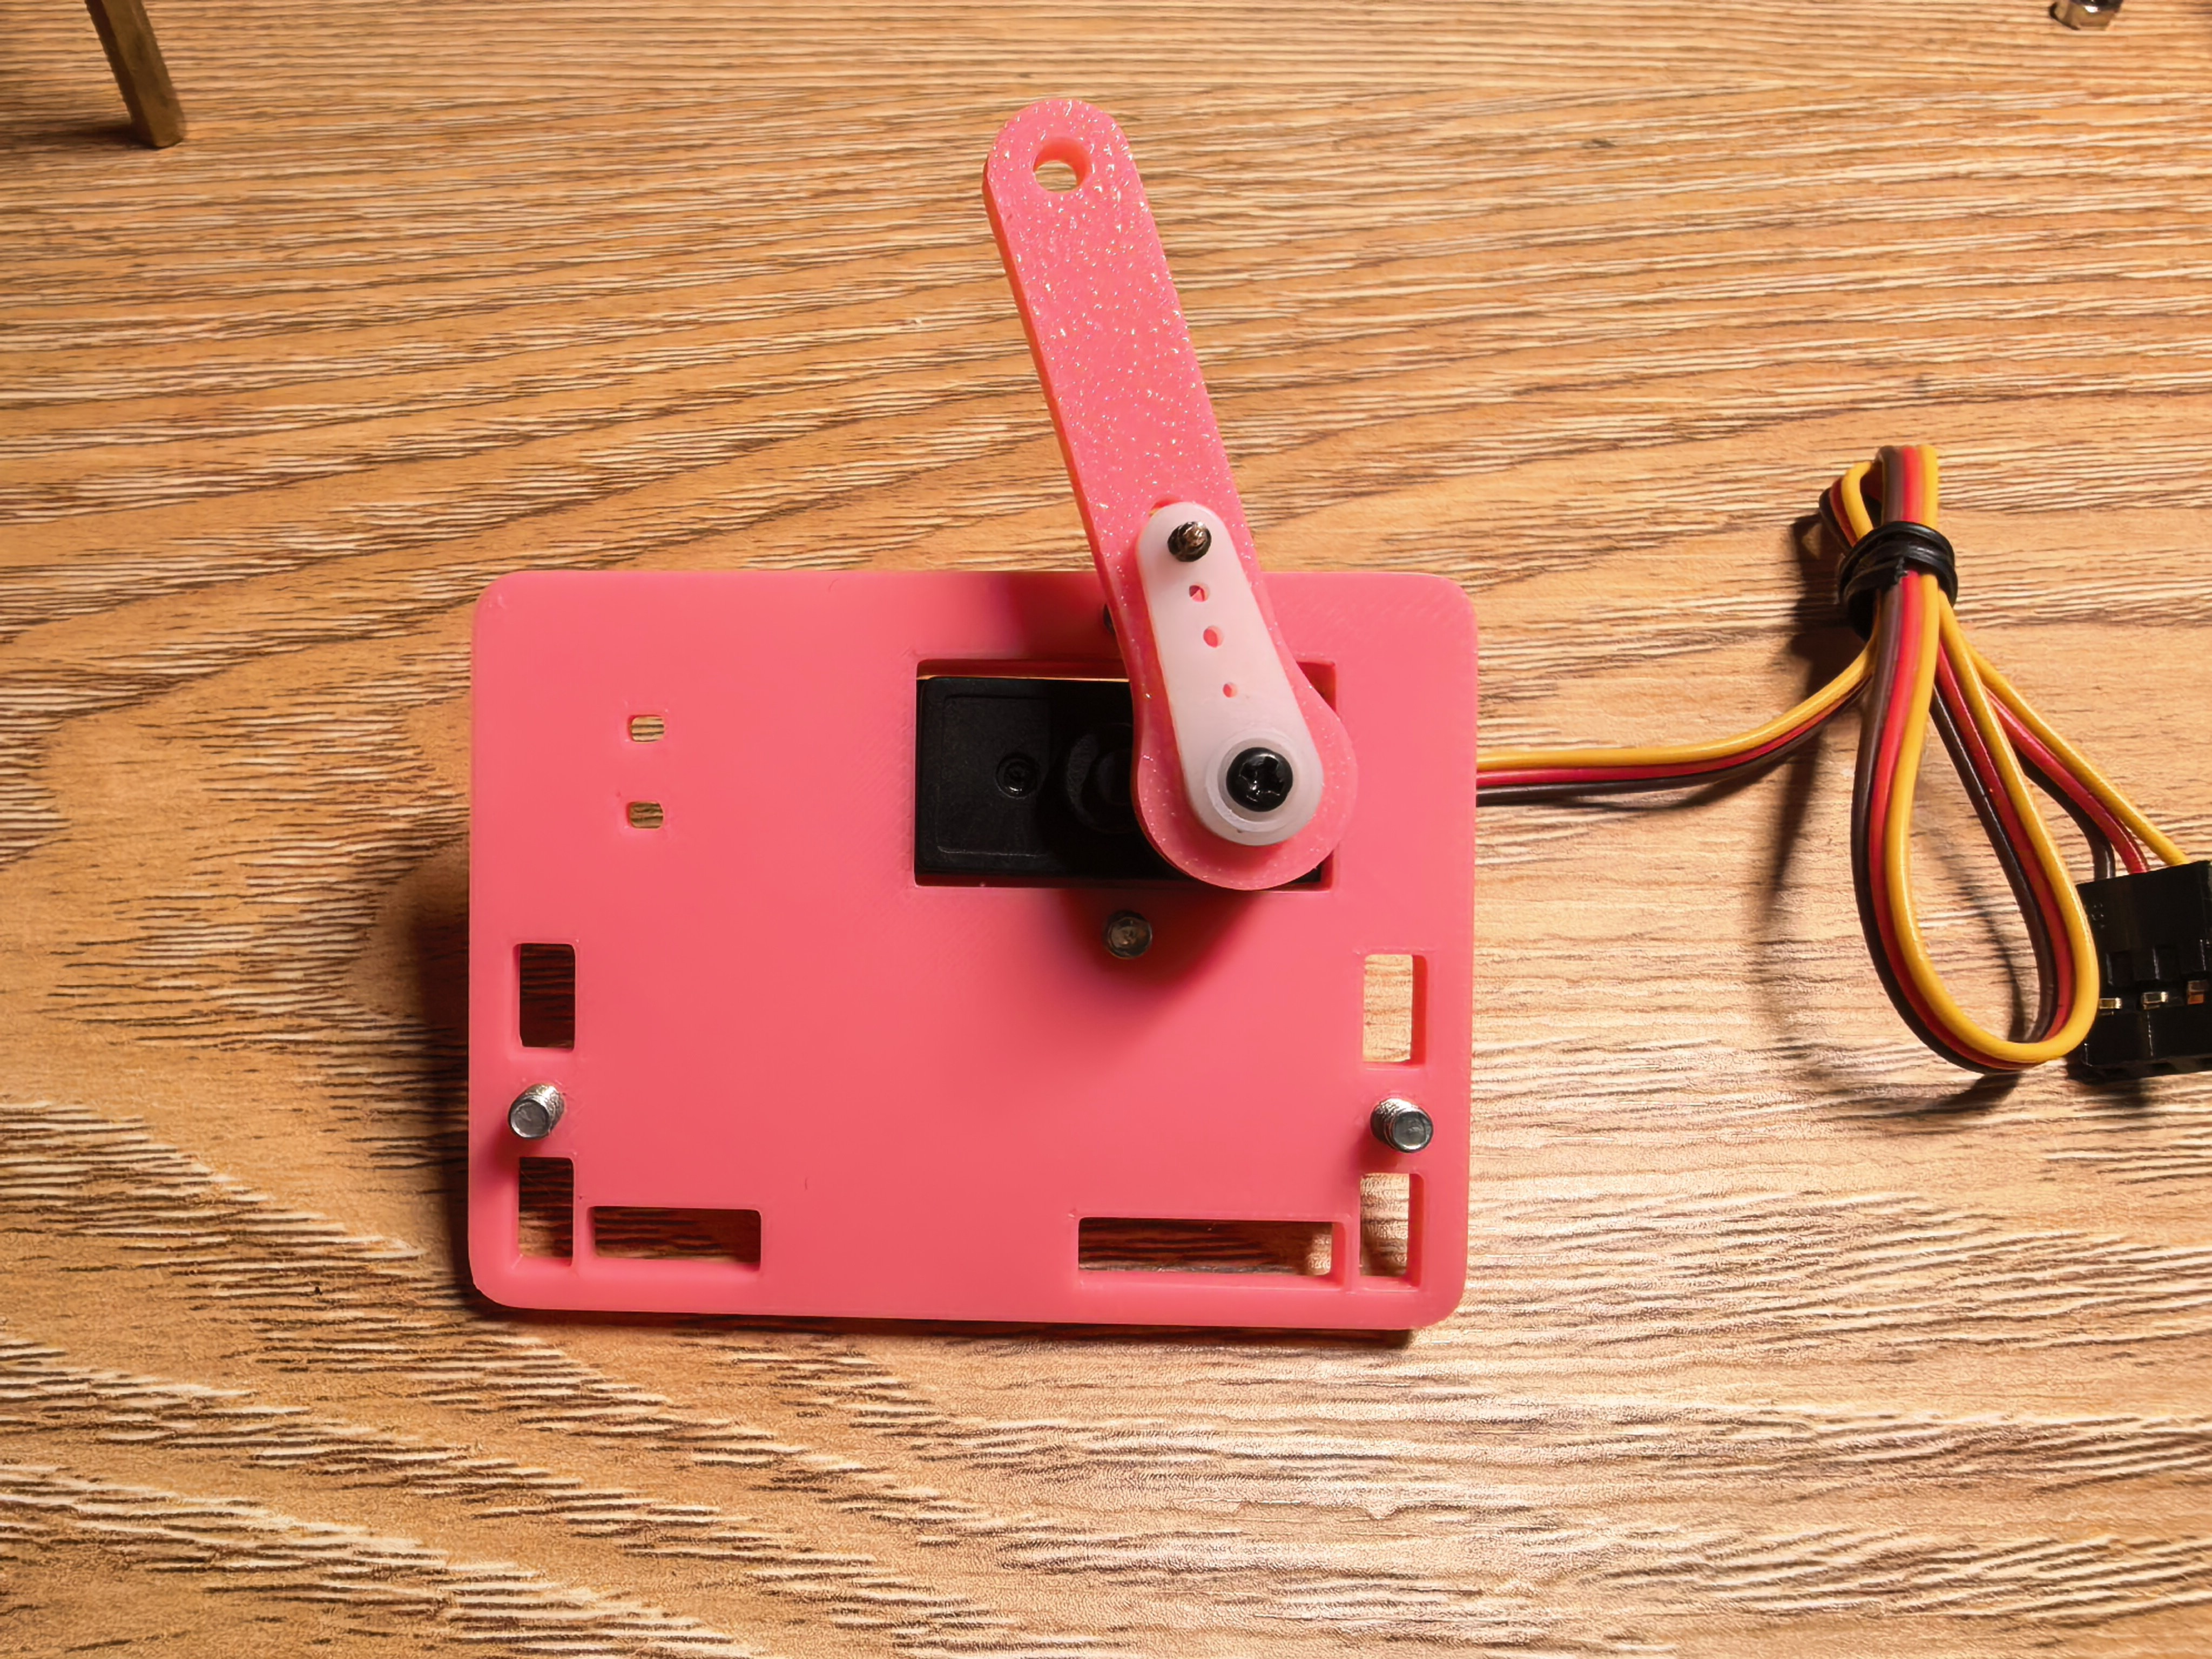
\includegraphics[width=\linewidth]{IMG_20260301_122523.jpg}
        \caption{小臂舵机安装}
        \label{fig:smallarm}
    \end{minipage}
    \hfill
    \begin{minipage}[b]{0.45\textwidth}
        \centering
        \includegraphics[width=\linewidth]{IMG_20260301_130007.jpg}
        \caption{舵机臂呈 V 型}
    \end{minipage}
\end{figure}

\begin{enumerate}
    \setcounter{enumi}{1}
    \item 将侧壁安装到转台上。
    \item \textbf{如果前面步骤正常安装，这里两个舵机臂应该呈 V 型}（假如装上去之后没有转的话）。
\end{enumerate}

\newpage
\section{安装夹爪}
\textbf{注意：舵机使用防堵转舵机！同样记得回到中立位置！}

\begin{enumerate}
    \item 按照图 \ref{fig:claw} 位置安装舵机臂和齿轮（注意舵机臂朝下、爪子打开），并可以直接装完夹爪的所有零件。
    \item \textbf{注意左右齿轮的正确配合，使夹爪左右两边是对称的！}
\end{enumerate}

% 图14 + 图15 并排
\begin{figure}[h!]
    \centering
    \begin{minipage}[b]{0.45\textwidth}
        \centering
        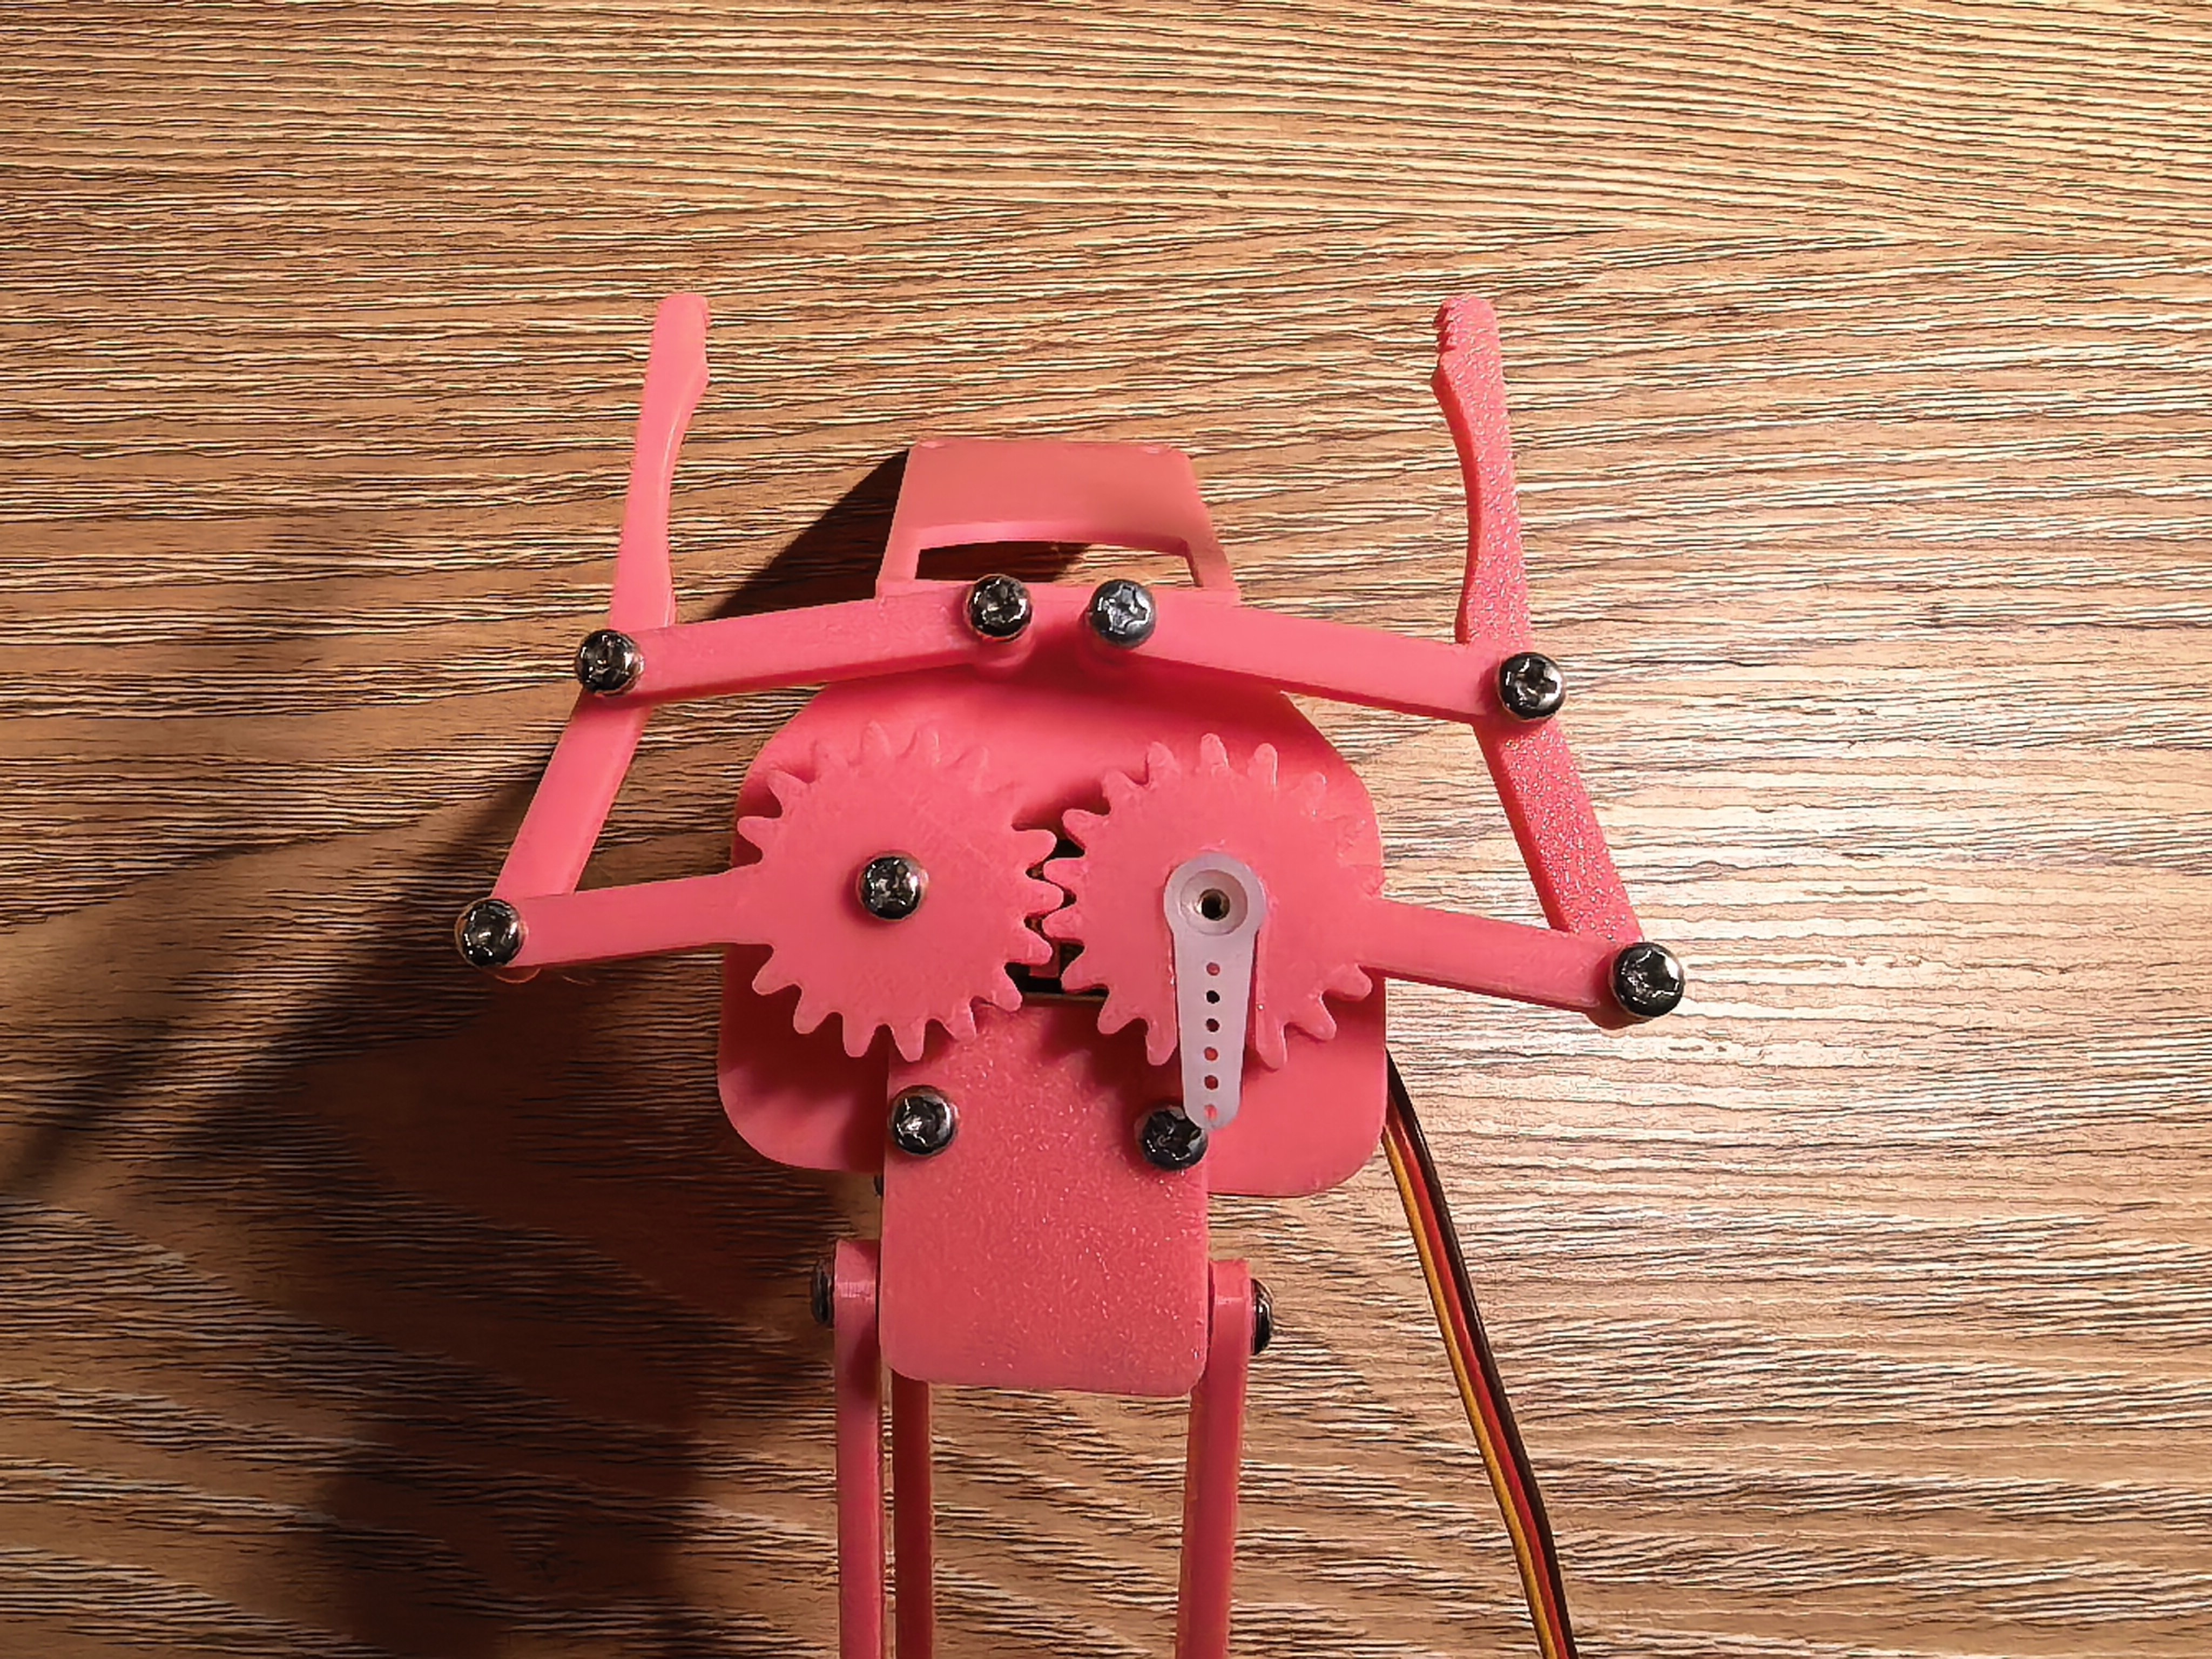
\includegraphics[width=\linewidth]{IMG_20260301_130818.jpg}
        \caption{夹爪安装}
        \label{fig:claw}
    \end{minipage}
    \hfill
    \begin{minipage}[b]{0.45\textwidth}
        \centering
        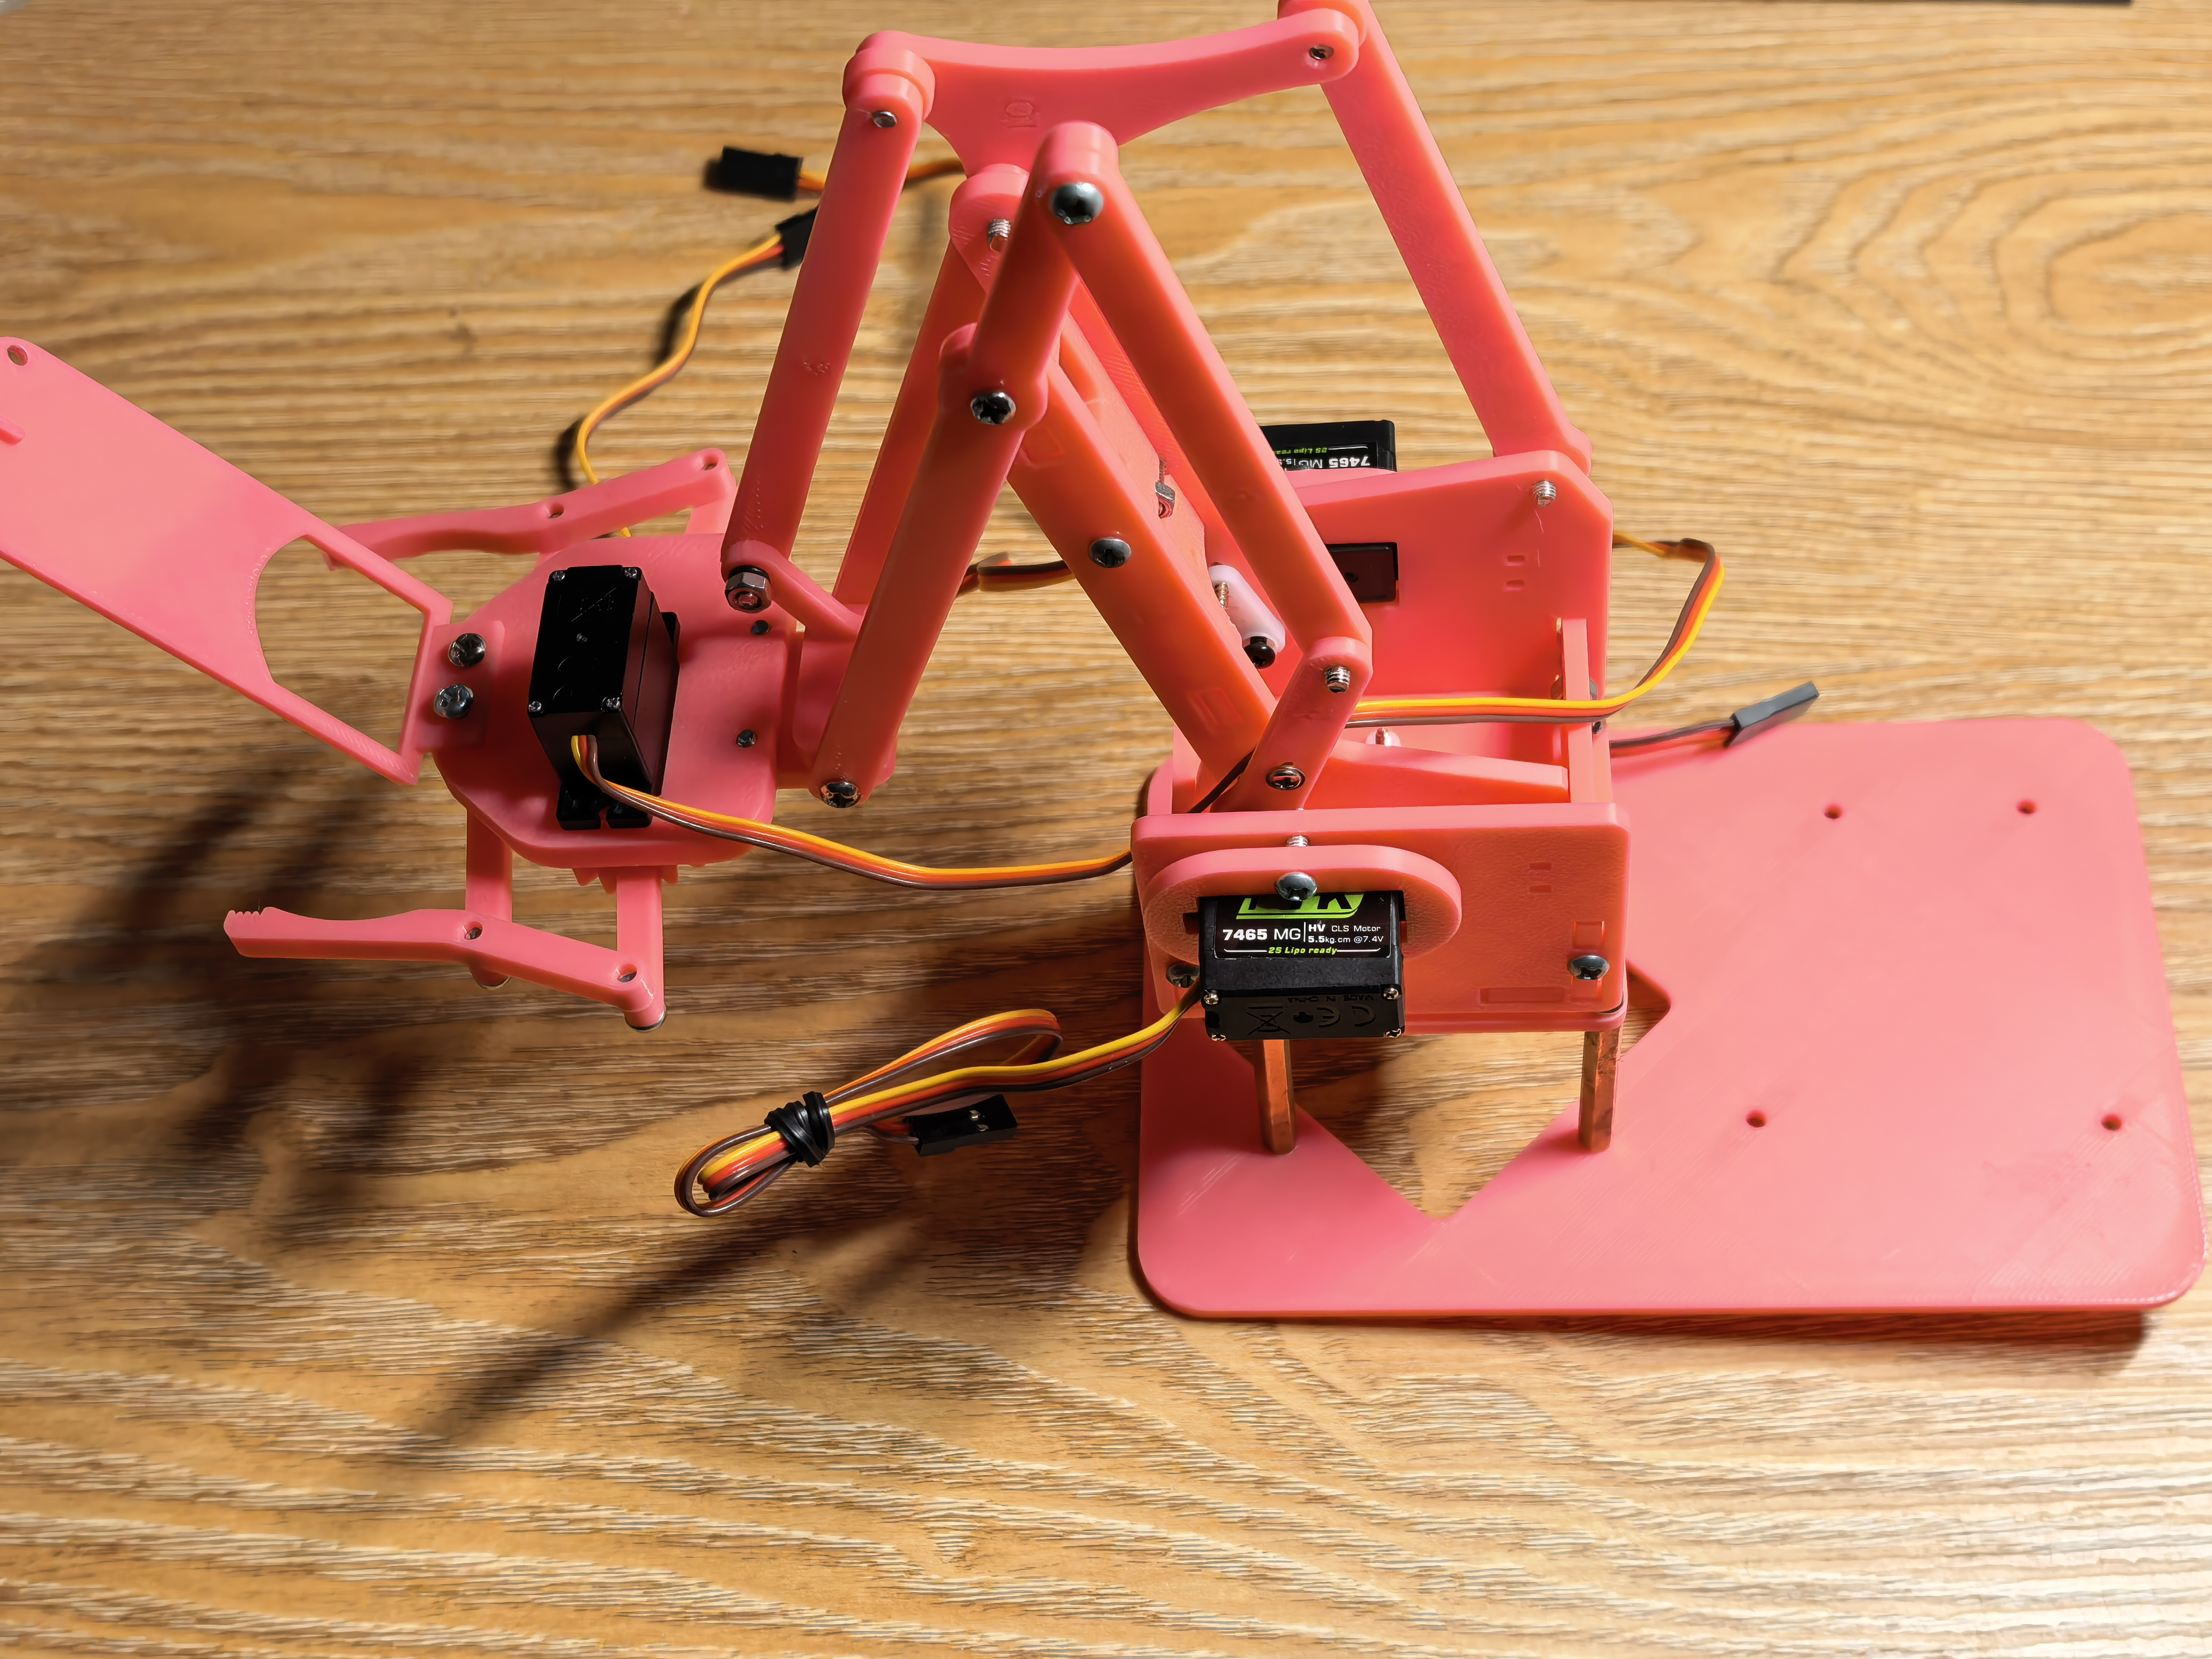
\includegraphics[width=\linewidth]{IMG_20260301_131818.jpg}
        \caption{剩余零件安装}
        \label{fig:15}
    \end{minipage}
\end{figure}

\section{完成剩余零件安装}
\begin{itemize}
    \item 可以按装配图直接完成剩下所有零件的安装！
    \item \textbf{注意：} 安装底座时将印有"ZJUSRA"字样的一面朝上！（图 \ref{fig:15} 中底座零件没有 ZJUSRA 字样，但孔朝向是对的）
\end{itemize}

\end{document}